% use UTF-8 encoding in editors such as TeXworks
% !TEX encoding = UTF-8 Unicode
% !TEX TS-program = pdflatex

\documentclass[%
    corpo=13.5pt,
    twoside,
%    stile=classica,
    oldstyle,
%    autoretitolo,
    tipotesi=magistrale,
    greek,
    evenboxes
]{toptesi}

\usepackage[utf8]{inputenc}% codifica d'entrata
\usepackage[T1]{fontenc}%    codifica dei font
\usepackage{lmodern}%        scelta dei font
\usepackage{listings}       % code listing
\usepackage{mathtools}      % math
\usepackage{eucal}          % math calligraphy
\usepackage{amsfonts}       % blackboard bold letters (like R for real values)
\usepackage{url}            % URLs usage: \url{https://example.com}
\usepackage{cite}           % cite bibtex entries
\usepackage{hyperref}       % internal references to text, chapters ecc

\def\UrlBreaks{\do\/\do-}   % break urls also using "-"


\usepackage{makecell}

\renewcommand\theadalign{bc}
\renewcommand\theadfont{\bfseries}
\renewcommand\theadgape{\Gape[4pt]}
\renewcommand\cellgape{\Gape[4pt]}


\usepackage{tabularx, booktabs, multirow, subcaption} % tables
\usepackage[table]{xcolor}
\newcolumntype{b}{X}
\newcolumntype{m}{>{\hsize=.5\hsize}X}
\newcolumntype{s}{>{\hsize=.4\hsize}X}
\newcolumntype{z}{>{\hsize=.3\hsize}X}
\newcolumntype{k}{>{\hsize=.2\hsize}X}
\newcolumntype{i}{>{\hsize=.2\hsize}>{\centering\arraybackslash}X}
\newcolumntype{u}{>{\hsize=.1\hsize}X}
\newcolumntype{Y}{>{\centering\arraybackslash}X} %centering

\newcommand*\rot{\rotatebox{90}} % multirow rotation

\usepackage{color}
\definecolor{gray}{rgb}{0.4,0.4,0.4}
\definecolor{darkblue}{rgb}{0.0,0.0,0.6}
\definecolor{cyan}{rgb}{0.0,0.6,0.6}
\definecolor{codebackground}{rgb}{0.95,0.95,0.92}


\lstset{
    basicstyle=\ttfamily,
    columns=fullflexible,
    showstringspaces=false,
    commentstyle=\color{gray}\upshape,
    aboveskip=12.5pt,
    belowskip=12.5pt
}

\lstdefinelanguage{XML}
{
  morestring=[b]",
  morestring=[s]{>}{<},
  morecomment=[s]{<?}{?>},
  stringstyle=\color{black},
  identifierstyle=\color{darkblue},
  keywordstyle=\color{cyan},
  morekeywords={xmlns,version}
}

% Vedere la documentazione toptesi-it.pdf per le
% attenzioni che bisogna usare al fine di ottenere un file
% veramente conforme alle norme per l'archiviabilità.

\usepackage{hyperref}
\hypersetup{%
    pdfpagemode={UseOutlines},
    bookmarksopen,
    pdfstartview={FitH},
    colorlinks,
    linkcolor={blue},
    citecolor={blue},
    urlcolor={blue}
  }

%%%%%%% Definizioni locali
\newtheorem{osservazione}{Osservazione}% Standard LaTeX
\ExtendCaptions{english}{Abstract}{Acknowledgements}



\begin{document}\errorcontextlines=9

% set english ad primary language
\english

%%%%%%%%%%%%%%%%%%%%
% BEGIN front page %
%%%%%%%%%%%%%%%%%%%%
\begin{ThesisTitlePage}*

\ateneo{Politecnico di Torino}
\nomeateneo{DEPARTMENT OF CONTROL AND COMPUTER ENGINEERING}
\CorsoDiLaureaIn{Master of Science in}
\corsodilaurea{Computer Engineering}
\TesiDiLaurea{Master Degree Thesis}

\titolo{Deep Learning on Academic Knowledge Graphs}
\sottotitolo{
    Predicting new facts in a novel semantic graph built
    on top of the Politecnico di Torino scholarly data
}

\CandidateName{Candidate}
\candidato{Giovanni \textsc{Garifo}}

\AdvisorName{Supervisors}
\relatore{Prof.~Antonio Vetrò}
\secondorelatore{Prof.~Juan Carlos De Martin}
\sedutadilaurea{\textsc{Academic~Year} 2018-2019}%

\logosede[6cm]{logopolito}
\end{ThesisTitlePage}
%%%%%%%%%%%%%%%%%%
% END front page %
%%%%%%%%%%%%%%%%%%


% offset rilegatura
%\setbindingcorrection{3mm}

\makeatletter
\newenvironment{miadedica}{
    \clearpage
    \if@twoside
        \ifodd\c@page\else\thispagestyle{empty}\null\clearpage\fi
    \fi
    \thispagestyle{empty}%
    \list{}{\labelwidth\z@
    \leftmargin.73\textwidth
    \parindent\z@
    \raggedright\LARGE\itshape}\item[]
    \normalsize
}

\begin{miadedica}
    To Monia\\
    To my Grandfather
\end{miadedica}


\paginavuota

%%%%%%%%%%%%%%%%%%%%%%%%%%%%%%%%%%%%%%%%%%%%%%%%%%%%%%%%%%%%%%%%%%%%%%%%%%%%%%%%
% -------------------------------- Abstract ---------------------------------- %
%%%%%%%%%%%%%%%%%%%%%%%%%%%%%%%%%%%%%%%%%%%%%%%%%%%%%%%%%%%%%%%%%%%%%%%%%%%%%%%%
\sommario

The publication and sharing of new research results is one of the
main goal of an academic institution. In recent years, many efforts have been
made to collect and organize the scientific knowledge through new,
comprehensive data repositories.
To achieve such goal new tools that are able not only to store data, but also to
describe them are needed.

Knowledge graphs are a particular class of graphs that are used to
semantically describe the human knowledge in a specific domain by linking
entities through labeled and directed edges.

In this work we are going to present a novel semantic graph built on top of the
scholarly data produced by the Politecnico di Torino (Polito), and how we
employed state-of-the-art machine learning techniques for the prediction
of new facts in the knowledge base.
Such graph, built by leveraging Semantic Web technologies, links together
publications, researchers, fields of study and scientific journals in order
to build a knowledge base that describes the Politecnico di Torino scientific
community.
We decided to call such new academic graph the \emph{Polito Knowledge Graph}.

The prediction of non-existent links between graph nodes is one of the
most challenging tasks in the field of statistical relational learning for graph
data, mainly because, in order to obtain meaningful predictions, the vector
representations of the entities must embed their semantic characteristics.
To accomplish such goal, we decided to employ a Deep Learning architecture derived
from the image recognition field and specifically adapted to the task of
representation learning for graph data.
Such architecture allowed us to obtain representations that have been
directly learnt from the graph structure itself, without requiring any prior
knowledge or feature engineering.
Leveraging such representations, we were able to obtain meaningful predictions
that we used to empower a recommendation system for the suggestion of useful
insights to the Polito researchers.

%%%%%%%%%%%%%%%%%%%%%%%%%%%%%%%%%%%%%%%%%%%%%%%%%%%%%%%%%%%%%%%%%%%%%%%%%%%%%%%%
% ------------------------------- acknowledgements --------------------------- %
%%%%%%%%%%%%%%%%%%%%%%%%%%%%%%%%%%%%%%%%%%%%%%%%%%%%%%%%%%%%%%%%%%%%%%%%%%%%%%%%
\ringraziamenti

I would like to express my deep gratitude to Giuseppe Futia, for his useful
advices, his support in the revision of this work and his enthusiastic
encouragement.

I would also like to thank all my colleagues and the directors of the
Nexa Center for Internet and Society, who supported me during my master
degree studies.
Special thanks should be given to Marco Conoscenti, Selina Fenoglietto and
Antonio Vetrò, for the support given during this years.

I also want to thank my family and friends, with a particular mention to
Angelo Cataldo, friend of a lifetime.

This work is dedicated to Monia Fontana, without whose support I would not
have been able to face the challenges that the life posed me in the latest
years, and to my Grandfather, Giovanni Rotolo, passed away shortly after
the start of my master degree, whom I hope to make proud by completing my
university studies.

% normalmente questa riga non serve ed e' commentata
\tablespagetrue\figurespagetrue
\indici

\mainmatter

%%%%%%%%%%%%%%%%%%%%%%%%%%%%%%%%%%%%%%%%%%%%%%%%%%%%%%%%%%%%%%%%%%%%%%%%%%%%%%%%
% ---------------------------- Introduction ---------------------------------- %
%%%%%%%%%%%%%%%%%%%%%%%%%%%%%%%%%%%%%%%%%%%%%%%%%%%%%%%%%%%%%%%%%%%%%%%%%%%%%%%%
\chapter{Introduction}

\section{Motivation}

Graphs are used to empower some of the most complex IT services available
today, an example among all is the Google search engine\footnote{\url{https://blog.google/products/search/introducing-knowledge-graph-things-not/}}.
Graphs can be used to represent almost any kind of information, and they are
particularly capable of representing the structure of complex systems and
describe the relationships between their elements.

Over the last decade, much effort has been put in trying to leverage the power
of graphs to represent human knowledge and to build search tools capable of
querying and understanding the semantic relations within them.
RDF\footnote{The Resource Description Framework will be introduced in
section \ref{subsec:semanticweb}} graphs are a
particular class of graphs that can be used to build knowledge
bases. Ontologies are used to shape such knowledge repositories, in order to
have a semantically coherent representation of the domain knowledge.
Given a domain and an ontology, RDF graphs allows to build a structured
representation of the knowledge in such domain.

Modern machine learning techniques can be used to mine latent information
from such graphs. One of the main challenges in this field is how to learn
meaningful representations of entities and relations that embed
the underlying knowledge. Such representations can then be used to evaluate
new links within the graph or to classify unseen nodes.
Deep learning techniques have proved to be first class citizens when
dealing with representation learning tasks, being able to learn latent
representations without any prior knowledge other than the graph structure.


\section{Goal and Contribution}

% issue
Knowledge sharing is one of the main goals of research organizations. In
particular, universities are among the most interested in making publicly
available their research results. Today most universities have embraced the Open
Science movement, making their scientific publications publicly available
through web portals.

An example of such tools is IRIS\footnote{\url{https://iris.polito.it/}}, which
stores all the scientific papers produced by the Politecnico di Torino,
publicly sharing them through Open Access.
IRIS allows to explore the published papers by searching for a field of study,
matching it with the keywords inserted by the authors of the publications.
This implementation has some limitations: being inserted by the authors, there
could be more keywords that refers to the same scientific topic.
Moreover, the author may have inserted acronyms or misspelled some words.
The consequence is that the search engine of IRIS is unable to correctly
retrieve all the publications about a specific research topic, because the
system cannot match the searched field of study with an unambiguous
\emph{semantic entity}, but only with character strings that are not
uniquely identified or semantically linked each other, and also prone to
lexical errors.

% goal
Our goal is to overcome such limitations and enabling new possibilities for
exploring and obtaining insights about the scientific community of the
Politecnico di Torino. A new semantic-empowered search engine can be
one of the possible solutions to obtain this results, allowing for coherent and
precise results to be retrieved.
At the foundations of this new semantic search engine there must be a data
structure capable of representing semantic relations and concepts. Once such
knowledge base of the scholarly data is obtained, it can be enhanced and
completed by automatically extracting latent information through the use of
advanced machine learning algorithms.

% contribution
In the next chapters we are going to present a newly built structured and
semantically coherent representation of the scholarly data produced by the
Politecnico di Torino, and how implicit facts can be automatically
extracted from such knowledge repository by leveraging knowledge base
completion techniques, implemented by means of an advanced link prediction
algorithm.



%%%%%%%%%%%%%%%%%%%%%%%%%%%%%%%%%%%%%%%%%%%%%%%%%%%%%%%%%%%%%%%%%%%%%%%%%%%%%%%%
% ------------------------------- Background --------------------------------- %
%%%%%%%%%%%%%%%%%%%%%%%%%%%%%%%%%%%%%%%%%%%%%%%%%%%%%%%%%%%%%%%%%%%%%%%%%%%%%%%%
\chapter{Background}

\section{Semantic Web}

\subsection{From a Web of Contents to a Web of Data}

The World Wide Web has been developed as a tool to easily access
documents and to navigate through them by following hyperlinks.
This simple description already resembles the structure of a graph: we can
think of documents as nodes and hyperlinks as edges. The unstoppable growth
of the \emph{Web graph} led to the raise of new tools to explore such
complexity. Search engines have been developed to easily navigate such a
giant graph. First approaches were based on analytics evaluations,
such as the number of times a document has been linked, as in the case of the
PageRank \cite{page1999} algorithm developed by Google.
\newline

The Web rapidly became one of the most innovative technology ever built,
allowing to retrive information quickly and easily as never before.
The next evolutionary step has been to think about a Web not only exploitable by
human beings but also by machines. In order to build such a comprehensive
system, where information can be not only machine-readable, but
machine-understandable, the World Wide Web had to move from a web of content, to
a web of data.
\newline

The World Wide Web Consortium (W3C) introduced the Semantic Web as an extention
to the prior standard of the WWW. Its primary goal has been
to define a framework to describe and query semantic information contained
in the documents available on the Web, so as to allow machines to understand
the semantic information contained in web pages. In the vision of Tim
Berners-Lee, the father of WWW, this would bring to the transition from a
World Wide Web to a Giant Global Graph\footnote{\url{https://web.archive.org/web/20160713021037/http://dig.csail.mit.edu/breadcrumbs/node/215}},
where a web page contains metadata that provides to a machine the needed
information to understand the concepts and meanings expressed in it.


\subsection{The Semantic Web Building Blocks}
\label{subsec:semanticweb}

The three key components of the Semantic Web standard are:
\begin{enumerate}
\item OWL: the Web Ontology Language\cite{mcguinness2004}
\item RDF: the Resource Description Framework\cite{lassila1998}
\item SPARQL: The SPARQL Protocol and RDF Query Language\cite{ducharme2013}
\end{enumerate}
\bigskip

OWL is a language used to define ontologies. In this context, an ontology
is defined as a collection of concepts, relations and constraints between
these concepts that describes an area of interest or a domain.
OWL allows to classify things in terms of their meaning by describing
their belonging to classes and subclasses defined by the ontology: if
a thing is defined as member of a class, this means that it shares the
same semantic meaning as all the other members of such class. The result of
such classification is a taxonomy that defines a hierarchy of how things
are semantically interrelated in the domain under analysis.
The instances of OWL classes are called individuals, and can be related
with other individuals or classes by means of properties. Each individual
can be characterized with additional information using literals, that
represent data values like strings, dates or integers.
\newline

The Resource Description Framework defines a standard model for the
description, modelling and interchange of resources on the Web.

The first component of the framework is the \emph{RDF Model and Syntax},
which defines a data model that describes how the RDF resources should be
represented. The basic model consist of only three object types: resource,
property, and statement.
A resource is uniquely identified by an Uniform Resource Identifier (URI).
A property can be both a resource attribute or a relation between resources.
A statement describes a resource property, and is defined as a triple
between a subject (the resource), a predicate (the property) and an
object (a literal or another resource).

The second component of the framework is the \emph{RDF Schema} (RDFS),
that defines a basic vocabulary for describing RDF resources and the
relationships between them. Many of the vocabularies and ontologies available
today are built on top of RDFS, such as the Friend of a Friend (FOAF)
ontology \cite{brickley2007}, for describing social networks, or the one
maintained by the Dublin Core Metadata Initiative \cite{weibel1998}, that
defines common terms and relations used in the definition of metadata for
digital resources.

\begin{figure}[ht]
\centering
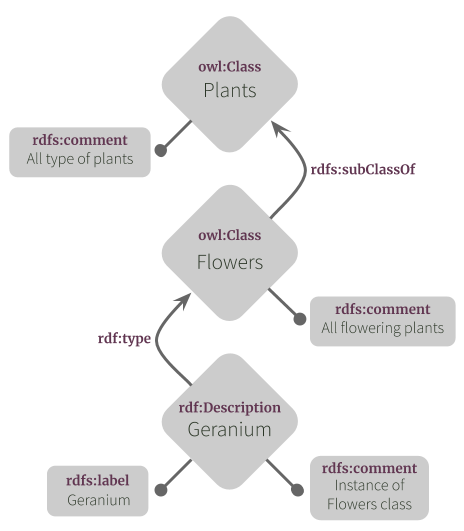
\includegraphics[scale=0.6]{img/owl-ontology-example.png}
\caption{An example of ontology defined using OWL and RDF Schema.}
\label{fig:owl-ontology-example}
\end{figure}

SPARQL is a query language for triplestores, a class of Database
Management Systems (DBMS) specialized in storing RDF databases. Such DBMS
often expose endpoints that can be used to query the database and obtain
results. Given the complexity of the stored data, the query language has
been designed to be as simple as possible, for instance by allowing the use
of variables, whose definition is preceded by a question mark.

The syntax of SPARQL is heavily derived from SQL, with some
minor adaptations to be more suited for querying graph data. The
following is an example of query which selects all the labels
(human-readable description of a resource) of all the entities that
match the given resource type.

\begin{lstlisting}[
        language=sparql,
        frame=single,
    ]
    PREXIF plants:<http://example.org/plants/>

    SELECT ?name
    WHERE {
        ?subject rdf:type plants:flowers .
        ?subject rdfs:label ?name .
    }
\end{lstlisting}

\subsection{Knowledge Bases as Knowledge Repositories}

% table: comparison of some of the biggest existing KG
\begin{table}
    \footnotesize
    \centering
    \caption{
        Comparison of some of the biggest industry-scale knowledge graphs
        developed to this date. Table adapted from \cite{noy2019}.
    }
    \label{tab:kg-comparison}

    \begin{tabularx}{1.0\textwidth}{ s b b m }
            \toprule
        & \textbf{Data model} & \textbf{Graph size} & \textbf{Development stage} \\
            \midrule
        \textbf{Microsoft} & Entities, relations and attributes defined in an ontology. & 2 billion entities and 55 billion facts. & Actively used in products. \\
            \midrule
        \textbf{Google} & Strongly typed entities, relations with domain and range inference. & 1 billion entities, 70 billion assertions. & Actively used in products. \\
            \midrule
        \textbf{Facebook} & All of the attributes and relations are structured and strongly typed. & 50 million primary entities, 500 million assertions. & Actively used in products. \\
            \midrule
        \textbf{eBay} & Entities and relation, well-structured and strongly typed. & 100 million products, more than 1 billion triples. & Early stages of development. \\
            \midrule
        \textbf{IBM} & Entities and relations with evidence information associated with them. & Various sizes. Proven on scales documents >100 million, relationships >5 billion, entities >100 million. & Actively used in products and by clients. \\
            \bottomrule
    \end{tabularx}
\end{table}

Even though the raise of the Semantic Web has suffered a slowdown in its growth
due to the complexity of its vision, many new projects were born from its
enabling technologies. Efforts have been put by profit and
non-profit organizations in trying to build complex knowledge repositories
starting from the knowledge already available in the Web. An example among all
is the DBpedia\footnote{\url{https://wiki.dbpedia.org/}} project, which
developed a structured knowledge base from the semi-structured data available on
Wikipedia.
Another example is the
\emph{Google Knowledge Graph}\footnote{\url{https://blog.google/products/search/introducing-knowledge-graph-things-not/}},
which is used to enhance the Google search engine and virtual assistant
capabilities, allowing to retrieve punctual information about everything that
has been classified in its ontology and described in its knowledge base, or
the \emph{Open Academic Graph}\footnote{\url{https://www.openacademic.ai/oag/}},
a Scientific Knowledge Graph that collects more then three hundred million
academic papers. A comparison between some of the biggest knowledge graphs
developed to this date is available in Table \ref{tab:kg-comparison}.

From an implementation perspective, knowledge bases can be created by defining
an ontology and a vocabulary for a specific domain of knowledge using OWL and
RDF Schema, and then by describing the concepts of such domain using the
RDF Model and Syntax.
The RDF document obtained can then be stored in a triplestore and queryed
using SPARQL.
The main effort in building knowledge bases is to have a correct understanding
and prior knowledge of the domain of interest, to avoid the risk of
mischaracterize or misrepresent concepts.

\begin{figure}[h]
    \centering
    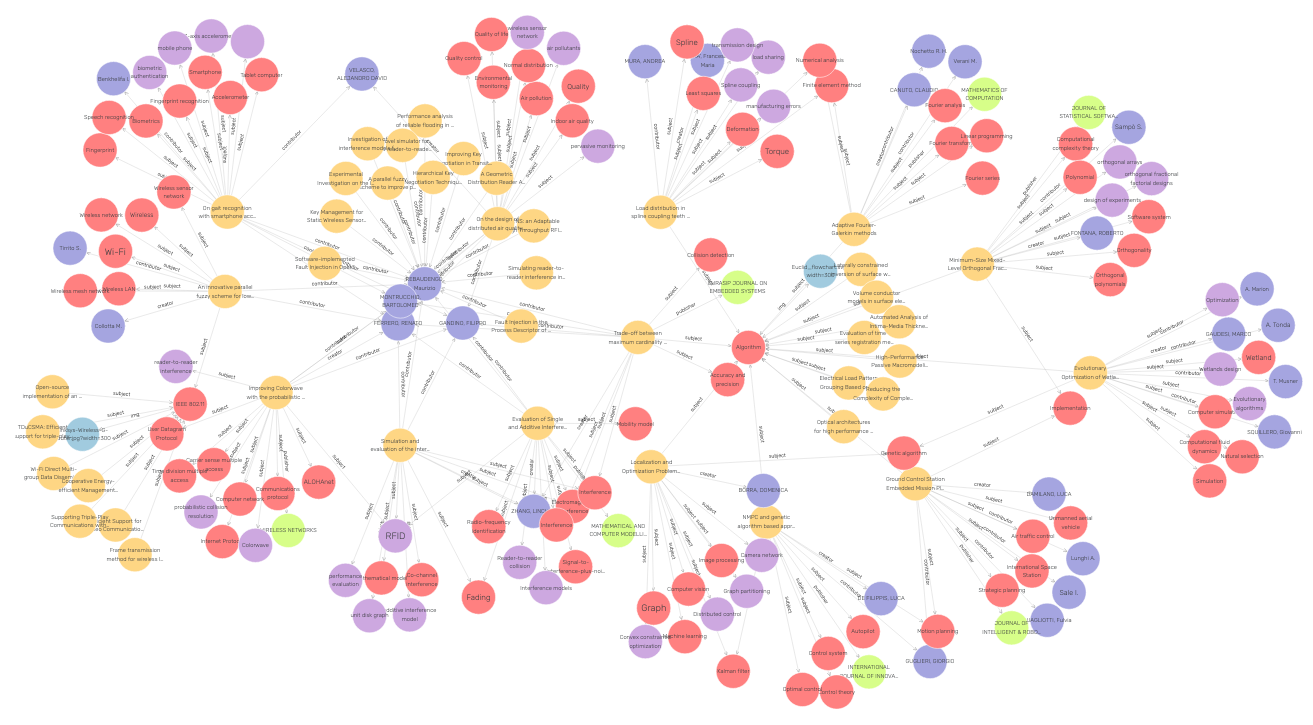
\includegraphics[scale=0.4]{img/geranium-knowledge-base-example.png}
    \caption{An extract of the Polito Knowledge Graph whose details will be
    described in section \ref{sec:buildingpkg}.}
    \label{fig:geranium-knowledge-base-example}
\end{figure}

If all the requirements and precautions are met, a well formed knowledge base may
prove to be a critical resource for an organization. It permits to
build new services upon it, and also to improve the existing knowledge inside
the organization by performing reasoning upon the available knowledge, in order
to derive implicit facts starting from the existing entities and relationships.
Another field of applications is the development of Expert Systems\footnote{\url{https://en.wikipedia.org/wiki/Expert_system}},
AI software that emulates the behavior of a human decision-making process by
navigating the knowledge base and taking decisions like in a rule-based system.

Today's knowledge bases are commonly composed of tens of
thousands nodes and by hundreds of thousands of edges.
Considering such dimensions, storing and querying giant graphs requires
the adoption of
specialized DBMS that are capable of efficiently store and query the RDF
input representation. Moreover, performing analysis and gathering statistics
from such giant graphs requires the adoption of highly efficient algorithms in
order to retrieve the desired output in an acceptable time.

The availability of such a complex and informative data structure leads
to the opening of interesting scenarios, especially when thinking about
the latent information that can be extracted from it. In
fact, a knowledge base is a structured representation of the
human knowledge in a specific field, thus its comprehensiveness is restricted
by the human understanding.


\section{Learning on Graphs}
\label{sec:learninggraphs}

\subsection{Representation Learning}

Machine learning (ML) algorithms are used to learn models from the
available data, with the final goal to obtain a set of parameters
that are fine-tuned to identify seen characteristics in the data
used for training. The obtained models can be used to
recognize unseen inputs by leveraging the knowledge embedded
in such parameters.
ML algorithms require the input data to be available in a
machine-understandable vector representation. An important task
in the ML field is the learning of such representations, task known
as representation learning.

Natural Language Processing is one of the research branches that in
the past years has made a great use of machine learning algorithms both for
language recognition and for embedding words meaning into words
vectors.
One of the most successful algorithms when dealing with representation learning
of words is Word2Vec \cite{mikolov2013}, where the model obtained is trained to
learn a vector representation for each word in a vocabulary.
In Word2Vec, the concept of meaning of a word is related to the context in
which such word is frequently used, so two words are recognized as similar if
they are used in similar contexts. In the vector space of the learnt
representations words that have similar meaning have an higher
cosine similarity\footnote{
    Cosine similarity is a heuristic method to measure the
    similarity between two vectors by computing the cosine of the angle between
    them:
    $similarity(A,B) = cos(\theta) = \frac{A \cdot B}{\Vert A \Vert \Vert B \Vert}$
}
with respect to the dissimilar ones.
For instance, the cosine similarity between the word vectors of "Man" and "King"
is roughly the same as the one between the words "Woman" and "Queen", since such
words are used in similar contexts. This has open up new scenarios for
language processing, since it allowed to perform vector
operations on words vectors, which brought interesting results.
An example can be seen in Figure \ref{fig:word2vec}.

\begin{figure}[t]
    \centering
    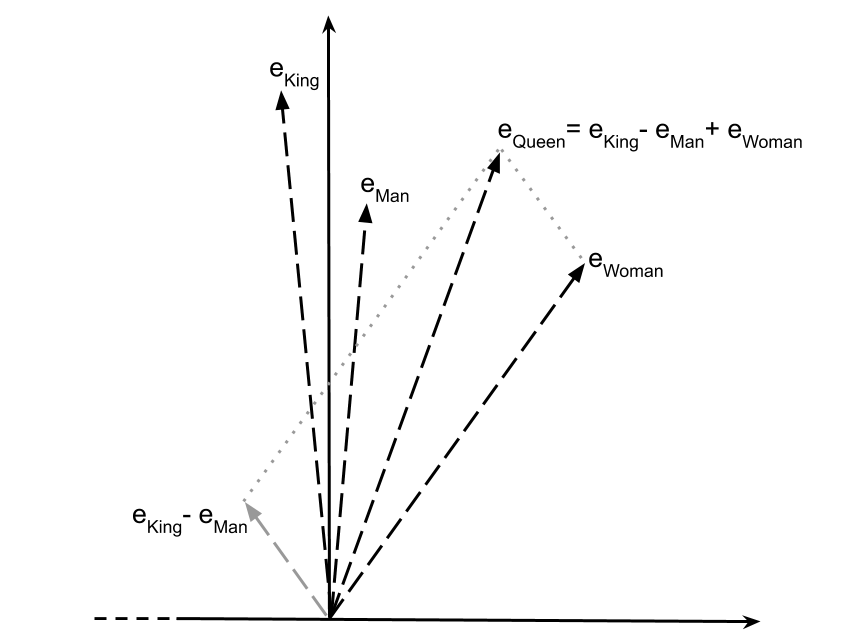
\includegraphics[scale=0.4]{img/word2vec.png}
    \caption{
        Word vectors allows to perform vector operations, the results
        obtained reflect the fact that Word2Vec is capable of embed the
        meaning of such words.
    }
    \label{fig:word2vec}
    \end{figure}

This idea of words characterized by the context in which they're used
can be generalized and applied to other fields of research, such as
the field of representation learning on graphs.

Graphs are composed of nodes and edges, and are used to describe complex
systems, such as social networks or the interactions in a molecular biology
system. To apply machine learning algorithms to such data structures
vector representations of nodes and edges are needed in order
to be able to learn from the available data and predict new facts.
Such vector representations are often referred to as \emph{embeddings} because
they should embed the characteristics of the graph nodes, so that similar nodes
have similar embeddings. For instance, in a scholarly knowledge base publications
with same authors and similar subjects should have similar embeddings.

Early approaches required these representations to be learned from feature
vectors that where handcrafted, task that required not
only a relevant amount of effort, but also a deep understanding of the domain
of interest. This has long been one of the main obstacles when dealing with
representation learning tasks, since who has knowledge of the domain and who
has to engineer the features were unlikely the same individual.


\subsection{Deep Learning on Graphs}

In the latest years a big shift towards deep architectures has been made
in machine learning, mainly thanks to the development of highly
parallelized architectures that are able to efficiently compute
at the hardware level vector and matrix multiplications, operations that
are at the basis of any machine learning task.
Deep Learning (DL) algorithms are able to extract relevant features from
raw data by applying simple mathematical operations, such as convolution, to
the input data.
An example of one of the most successful applications of DL is in
image recognition, where matrix representations of images are
convolved with self-trained filters that are able to
extract the relevant features needed to recognize patterns present
in the input images.

Deep learning techniques have proven to perform well also in the field of
representation learning for graph data.
As can be seen in figure \ref{fig:pixels-as-graph}, a digital image
is composed of pixels which can be thought of as nodes in a graph, where
each pixel is connected by an edge to its immediate neighbors. This suggests
that the techniques used when dealing with images can be adapted, with
some major changes, to the field of representation learning on graphs, but
also in other fields of research, such as learning on manifolds.

\begin{figure}[h]
    \centering
    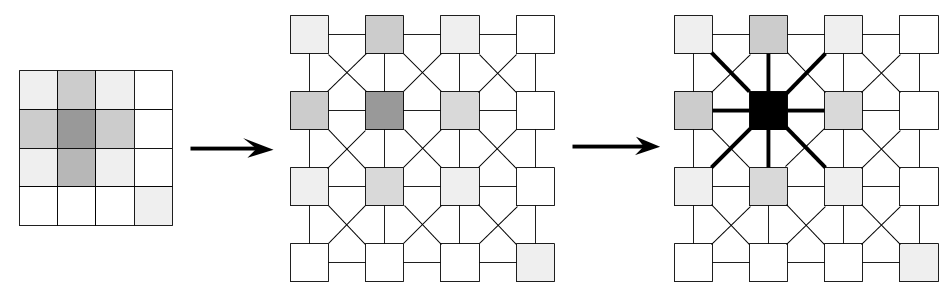
\includegraphics[scale=0.4]{img/pixels-as-graph.png}
    \caption{A digital image can be thought of as a graph.}
    \label{fig:pixels-as-graph}
\end{figure}

One of the issues when working with graph data is that commonly graphs
are built to describe complex systems, such as the knowledge of a
domain or field for knowledge graphs, and thus are composed of
a fairly high amount of nodes and edges. The matrices used to
store the graph structure can thus explode in dimensionality, becoming
impractical as input data. Moreover, graphs are not
regular structures with a given shape and size, such a matrix of pixels
for images, but they live in an irregular domain which led to highly
irregular structures.
The first issue can be solved by randomly sampling the graph at each
training epoch, the immediate drawback being that more than one epoch
is required to train over all graph nodes. The second issue can instead be
solved by adapting already existing algorithms to work on irregular domains.
One of the possible approaches, which has proven to work well, is
the one based on convolutions.

Graph Convolutional Networks (GCNs) \cite{kipf2016} are a class of
semi-supervised deep learning algorithms for graphs which are based on the
same convolution and backpropagation operations as the well known
Convolutional Neural Networks\cite{krizhevsky2012} (CNNs) used for feature
learning on images.
The main difference between CNNs and GCNs is in how the convolution is
performed, instead the backpropagation phase is the same as the one
used to update the parameters of CNNs, with a task-specific loss function.
In a CNN the input matrix of each network layer, which is the pixel matrix
of the input image for the first layer, is convolved with some layer-specific
convolutional filters, whose parameters are then updated during the
backpropagation phase.

GCNs works similarly by convolving at the \emph{l}-th layer
of the network the feature vector of each node with the feature
vectors of its \emph{l}-nearest neighbors by means of a convolutional filter.
This operation is done by applying the following transformation:

\begin{equation} \label{gcn1}
H^{(l+1)}=\sigma(\tilde{D}^{-1/2}\tilde{A}\tilde{D}^{-1/2}H^{(l)}W^{(l)})
\end{equation}

Where $H^{(l)} \in\mathbb{R}^{N \times d^{(l)}}$ is the nodes hidden
representation matrix, which is the output of the previous layer, with $N$ being
the number of nodes in the graph and $d^{(l)}$ being the dimensionality of
the current layer. For the first
layer, $H^{0}$ is equal to the input feature matrix $X$, where each row can be
initialized with the respective node feature or with a one-hot encoded vector.
For the last layer, $H^{(l+1)}$ is the embeddings matrix.
$\tilde{A}$ is an adjacency matrix of the graph that includes self loops.
$\tilde{D}$ is the node degree matrix of $\tilde{A}$ and is used to
normalize it.
$W^{l}\in\mathbb{R}^{d^{(l)} \times d^{(l+1)}}$ is the convolutional filter that
is shared among all nodes and is unique for each layer.
The shape of this filter will directly impact the dimensionality of the
embeddings obtained, in fact $H^{l+1}$ is shaped as a $N\times d^{(l+1)}$ matrix.
Finally, $\sigma$ is a non linear activation function, for instance $ReLU$.

Looking at the update rule of a single node embedding will make more clear how
the convolution is actually performed.
The forward rule to update the embedding of a single node at the $l$-th layer
of the network is the following:

\begin{equation} \label{gcn2}
    h^{(l+1)}_{i}=\sigma(\sum_{j\in\eta_{i}} \frac{1}{c_{i,j}}h_j^{(l)}W^{{(l)}})
\end{equation}

Where $\eta_i$ is the set of neighbors of node $i$, which contains the node
itself because of the added self loop, and $c_{ij}$ is a
normalization constant obtained from the multiplication between the adjancency
and degree matrices.
The updated feature vector $h^{(l+1)}_{i}$ of the node $i$ is
obtained by performing the following operations:

\begin{enumerate}
    \item The feature vectors $h_j^{(l)}$ of its neighbors are transformed by
        the matrix multiplication with the layer filter $W^{(l)}$.
    \item The resulting $1 \times d^{(l+1)}$ shaped features vectors
        are multiplied with the respective normalization constants and summed
        together.
    \item The non-linear function is applied to the result of the summation,
        obtaining the updated feature vector of the node $i$.
\end{enumerate}

Applying such transformations to all nodes, at the
$k$-th layer a node is represented by its transformed feature vector, which
embeds the structural information within the node's $k$-hop neighborhood.
As a consequence of this, the amount of layers of the network is an
hyperparameter that controls how much information from furthest nodes has to be
collected in each node embedding.
This represents a fundamental architectural difference between CNNs and GCNs:
while the former are commonly built by stacking a lot of layers, the latter
relies on architectures that are more wider, due to the dimensionality of the
graphs involved, and that consist of a fairly low amount of layers, in order to
characterize the nodes only by their immediate surroundings.


\begin{figure}[h]
    \centering
    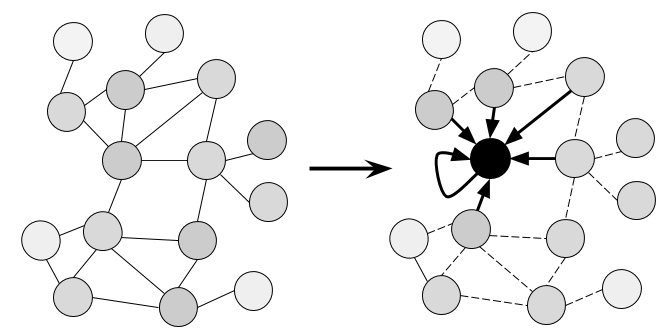
\includegraphics[scale=0.4]{img/gcn.png}
    \caption{Representation of a GCN updating the feature vector of the node \emph{0}
        by summing the convolved features of its adjacent nodes.}
    \label{fig:gcn}
\end{figure}

As a result of the propagation step each node embedding will be characterized by
its context, just like it happens in Word2Vec, but in a non-euclidean domain.
So for example, in a social graph where each person is characterized by its
friends, hobbies, places visited and so on, two people will have similar
embeddings if they are both linked to the same nodes, and so they share the
same interests and social connections.

The node embeddings obtained by applying a GCN or one of its variants can
then be used to perform some learning tasks on the graph, two examples are
the classification of unseen nodes or the link prediction of non-existent
edges. The latter is one of the most interesting tasks, since it allows to
complete the information contained in the graph by predicting unseen facts.

\subsection{Link Prediction on Knowledge Graphs}
\label{subsec:linkprediction}

Predicting new facts is one of the most common task in the field
of knowledge graph completion. The goal of such task is to predict new, unseen
triples that correspond to missing facts in the knowledge base, and that can be
later added to the graph.
Deep learning techniques for link prediction are based on the following two
main steps:

\begin{enumerate}
    \item Train an \emph{encoder} model
    that is able to embed the node features and produce meaningful embeddings.
    \item Apply a factorization model that act as a \emph{decoder}, which is
    used to score the unseen triples under evaluation.
\end{enumerate}

Deep learning techniques such as GCN can be exploited to obtain meaningful
node embeddings, but fall short when dealing with graphs where
nodes are connected by different relations (multi-relational graphs).
In fact, if we use a single layer GCN to obtain the embeddings of two nodes
that share the same neighborhood, but are connected to the neighbors via
different relations, we'll obtain almost the same embeddings, even if it's
clear that they do not share the same characteristics. For example in a
producer-consumer framework one node could be the producer while the other
the consumer, having both a common neighborhood of nodes
which are produced by the former and consumed by the latter.
If a GCN is used, the embeddings obtained would be very similar, even if
the two nodes clearly do not have the same role and do not belong to the
same class.

To overcome this limitation, changes to the basic GCN architecture have been
proposed, so to obtain models that works well when applied to multi-relational
graphs.
\newline

The Relational Graph Convolutional Network \cite{schlichtkrull2018} (R-GCN) is an
extension of GCNs which is focused on modeling multi-relational graphs composed
by labeled and directed edges, and thus is particularly capable of embedding
both nodes and relations of a knowledge graph.
R-GCN can be used for both link prediction and node classification tasks.

At an high level the R-GCN architecture can be seen as a special case of
the \emph{message passing framework} \cite{gilmer2017}, which groups together
under a common scheme most of the existing neural models for graph data.
The framework defines two major phases: a per-edge message computation and a
per-node message reduction.
In the first phase a function or linear transformation is applied to each edge
to obtain an edge-specific message.
Then, in the reduce phase, the embedding of each node is updated by aggregating
together all the messages of the incoming edges.

This two phases can be grouped together through the following equation:

\begin{equation}
    h_i^{(l+1)} = \sigma \left(
            \sum_{m\in{\CMcal{M}_i}} g_m(h_i^{(l)}, h_j^{(l)})
        \right)
\end{equation}

Where $\CMcal{M}_i$ is the set of incoming messages for node $i$ and
$g_m$ is a message specific transformation.
\newline

The idea behind the R-GCN is to have different set of parameters
for different relations.
At each step inside the network, the feature vector of a node is updated by
convolving its first neighbors features with a convolutional filter that is
different based on the kind of relation that connects the nodes.
The forward
rule to update the embedding of a node at the \emph{l}-th layer is the following:

\begin{equation}
    h^{(l+1)}_{i} = \sigma \left(
        W_0^{(l)}h_i^{(l)} + \sum_{r\in\CMcal{R}}\sum_{j\in\CMcal{N}_i^r}
        \frac{1}{c_{i,r}} W_r^{(l)} h_j^{(l)}
    \right)
\end{equation}

Where $h_i^{(l)}$ is the embedding (or, for the first layer, the input feature
vector) of the node \emph{i}, $W_0^{(l)}$ is the learnt kernel for the
self loop relation, $\CMcal{N}_i^r$ is the
set of indices of the neighbors of node \emph{i} under the relation
$r\in\CMcal{R}$, with $\CMcal{R}$ being the set of all the relations present in
the graph. $W_r^{(l)}\in\mathbb{R}^{d^{(l+1)}\times d^{(l)}}$ is the learnt
filter for the relation $r$. As for the GCN architecture, $\sigma$ is a non
linear activation function and $c_{i,r}$ is a normalization constant, commonly
initialized to $|\CMcal{N}_i^r|$.

From a message passing framework perspective, the message function (per-edge
transformation) is equal to the linear transformation $W_rh_j$, and the reduce
function (per-node transformation) is just the sum of
all the messages computed for the edges connected to each node.

As can be seen the update rule looks similar to the one for GCNs (\ref{gcn2}),
with the major difference that in the case of a R-GCN the filters used to
convolve the feature vectors of neighboring nodes are relation-specific, so the
number of filters at each layer will be equal to the number of relations inside
the graph. As a consequence, the kind of relation that connect the node
to its neighbors has an important role in determining the transformed node
embedding.

\begin{figure}[h]
    \centering
    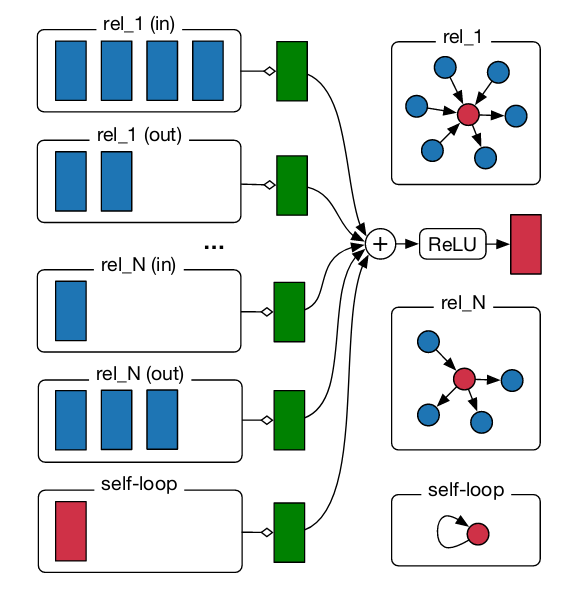
\includegraphics[scale=0.48]{img/rgcn-encoder.png}
    \caption{R-GCN encoder visualization. Image taken from \cite{schlichtkrull2018}.}
    \label{fig:rgcn-encoder}
\end{figure}

Some form of regularization is required in order to avoid overfitting on rare
relations, thus to obtain a more generalized model, and also to avoid
the rapid growth in the number of parameters of the network for
highly multi-relational graphs. One of the solutions proposed by the original
paper \cite{schlichtkrull2018} is to decompose each relation filter $W_r$
using basis decomposition:

\begin{equation}
    W_r^{(l)} = \sum_{b=1}^B a_{r,b}^{(l)} V_b^{(l)}
\end{equation}

This allows to store only the relation-specific coefficients and the basis,
which will be shared by all the relations.

The model obtained by training a R-GCN can then be used to build an encoder
that given as input a graph, gives as output the embeddings of all nodes and
the relations parameters. Then a factorization method can be used to
evaluate unseen facts inside the graph, exploiting the resulting embeddings.
Such methods are used as scoring functions in order to obtain, starting from
the entities embeddings, a real value that can be used to score the unseen
triples under evaluation.
\newline

DistMult \cite{yang2014} is one of the most common and simple factorization
methods used to score unseen triples. Given a triple $(s, p, o)$, where $s$
is the source node, $o$ is the destination node, and $r$ is the relation of the
edge that links the source to the destination, DistMult allows to compute
an associated real valued score as follows:

\begin{equation}
    score_{(s,r,o)} = f(s,r,o) = e_s^T R_r e_o
\end{equation}

Where $e_s$ and $e_o$ are the embeddings of the source and the destination node,
obtained by means of an encoder model like R-GCN, and
$R_r\in\mathbb{R}^{d \times d}$ is obtained by transforming the embedding
of the relation $r$ into a diagonal matrix. Such relation embedding is not
learnt by the R-GCN encoder, but is a randomly initialized vector that
represent the relation.

The score obtained by applying the factorization method above can then be used
to evaluate wether the triple $(s,r,o)$ is a good candidate to be added to the
graph: an high score has to be interpreted as a high confidence of the model
in the fact that the triple should belong to the knowledge base.



%%%%%%%%%%%%%%%%%%%%%%%%%%%%%%%%%%%%%%%%%%%%%%%%%%%%%%%%%%%%%%%%%%%%%%%%%%%%%%%%
% -------------------------- Approach and methodology ------------------------ %
%%%%%%%%%%%%%%%%%%%%%%%%%%%%%%%%%%%%%%%%%%%%%%%%%%%%%%%%%%%%%%%%%%%%%%%%%%%%%%%%
\chapter{Approach and Methodology}
\label{ch:approach}

This chapter introduces the architecture developed to build, enhance
and visualize the Polito Knowledge Graph (PKG), an academic RDF graph
built to organize in a structured and semantically coherent way the publications
produced by the researchers of the Politecnico di Torino. The graph
also includes publication-related entities, such as authors, journals,
and fields of study.

The architecture is composed of three main modules, that at an high level
can be seen as part of a producers-consumers architecture, where the former
produces the graph data, and the latter consumes it.

The architecture, which is shown in Figure \ref{fig:pipeline}, is structured
as a pipeline composed of the following three modules:

\begin{enumerate}
    \item The \emph{Builder}, which creates a first version of the
    RDF graph.
    \item The \emph{Enhancer}, which implements ML techniques to predict
    unseen facts. Such facts can then be added to the graph in order to
    complete the knowledge base.
    \item The \emph{Viewer}, a web application that allows to query
    and visualize the graph data.
\end{enumerate}

The \emph{Builder} act as producer taking as input the IRIS data
and producing a set of RDF statements that together composes the
Polito Knowledge Graph.
The \emph{Enhancer} act as both a producer and a consumer, given that it
takes as input the PKG and use it to predict unseen facts that can be
later added as new RDF statements.
The \emph{Viewer} consumes the graph by storing it a triplestore and exposing
a public web interface for querying and visualizing the data.


\begin{figure}[h]
    \centering
    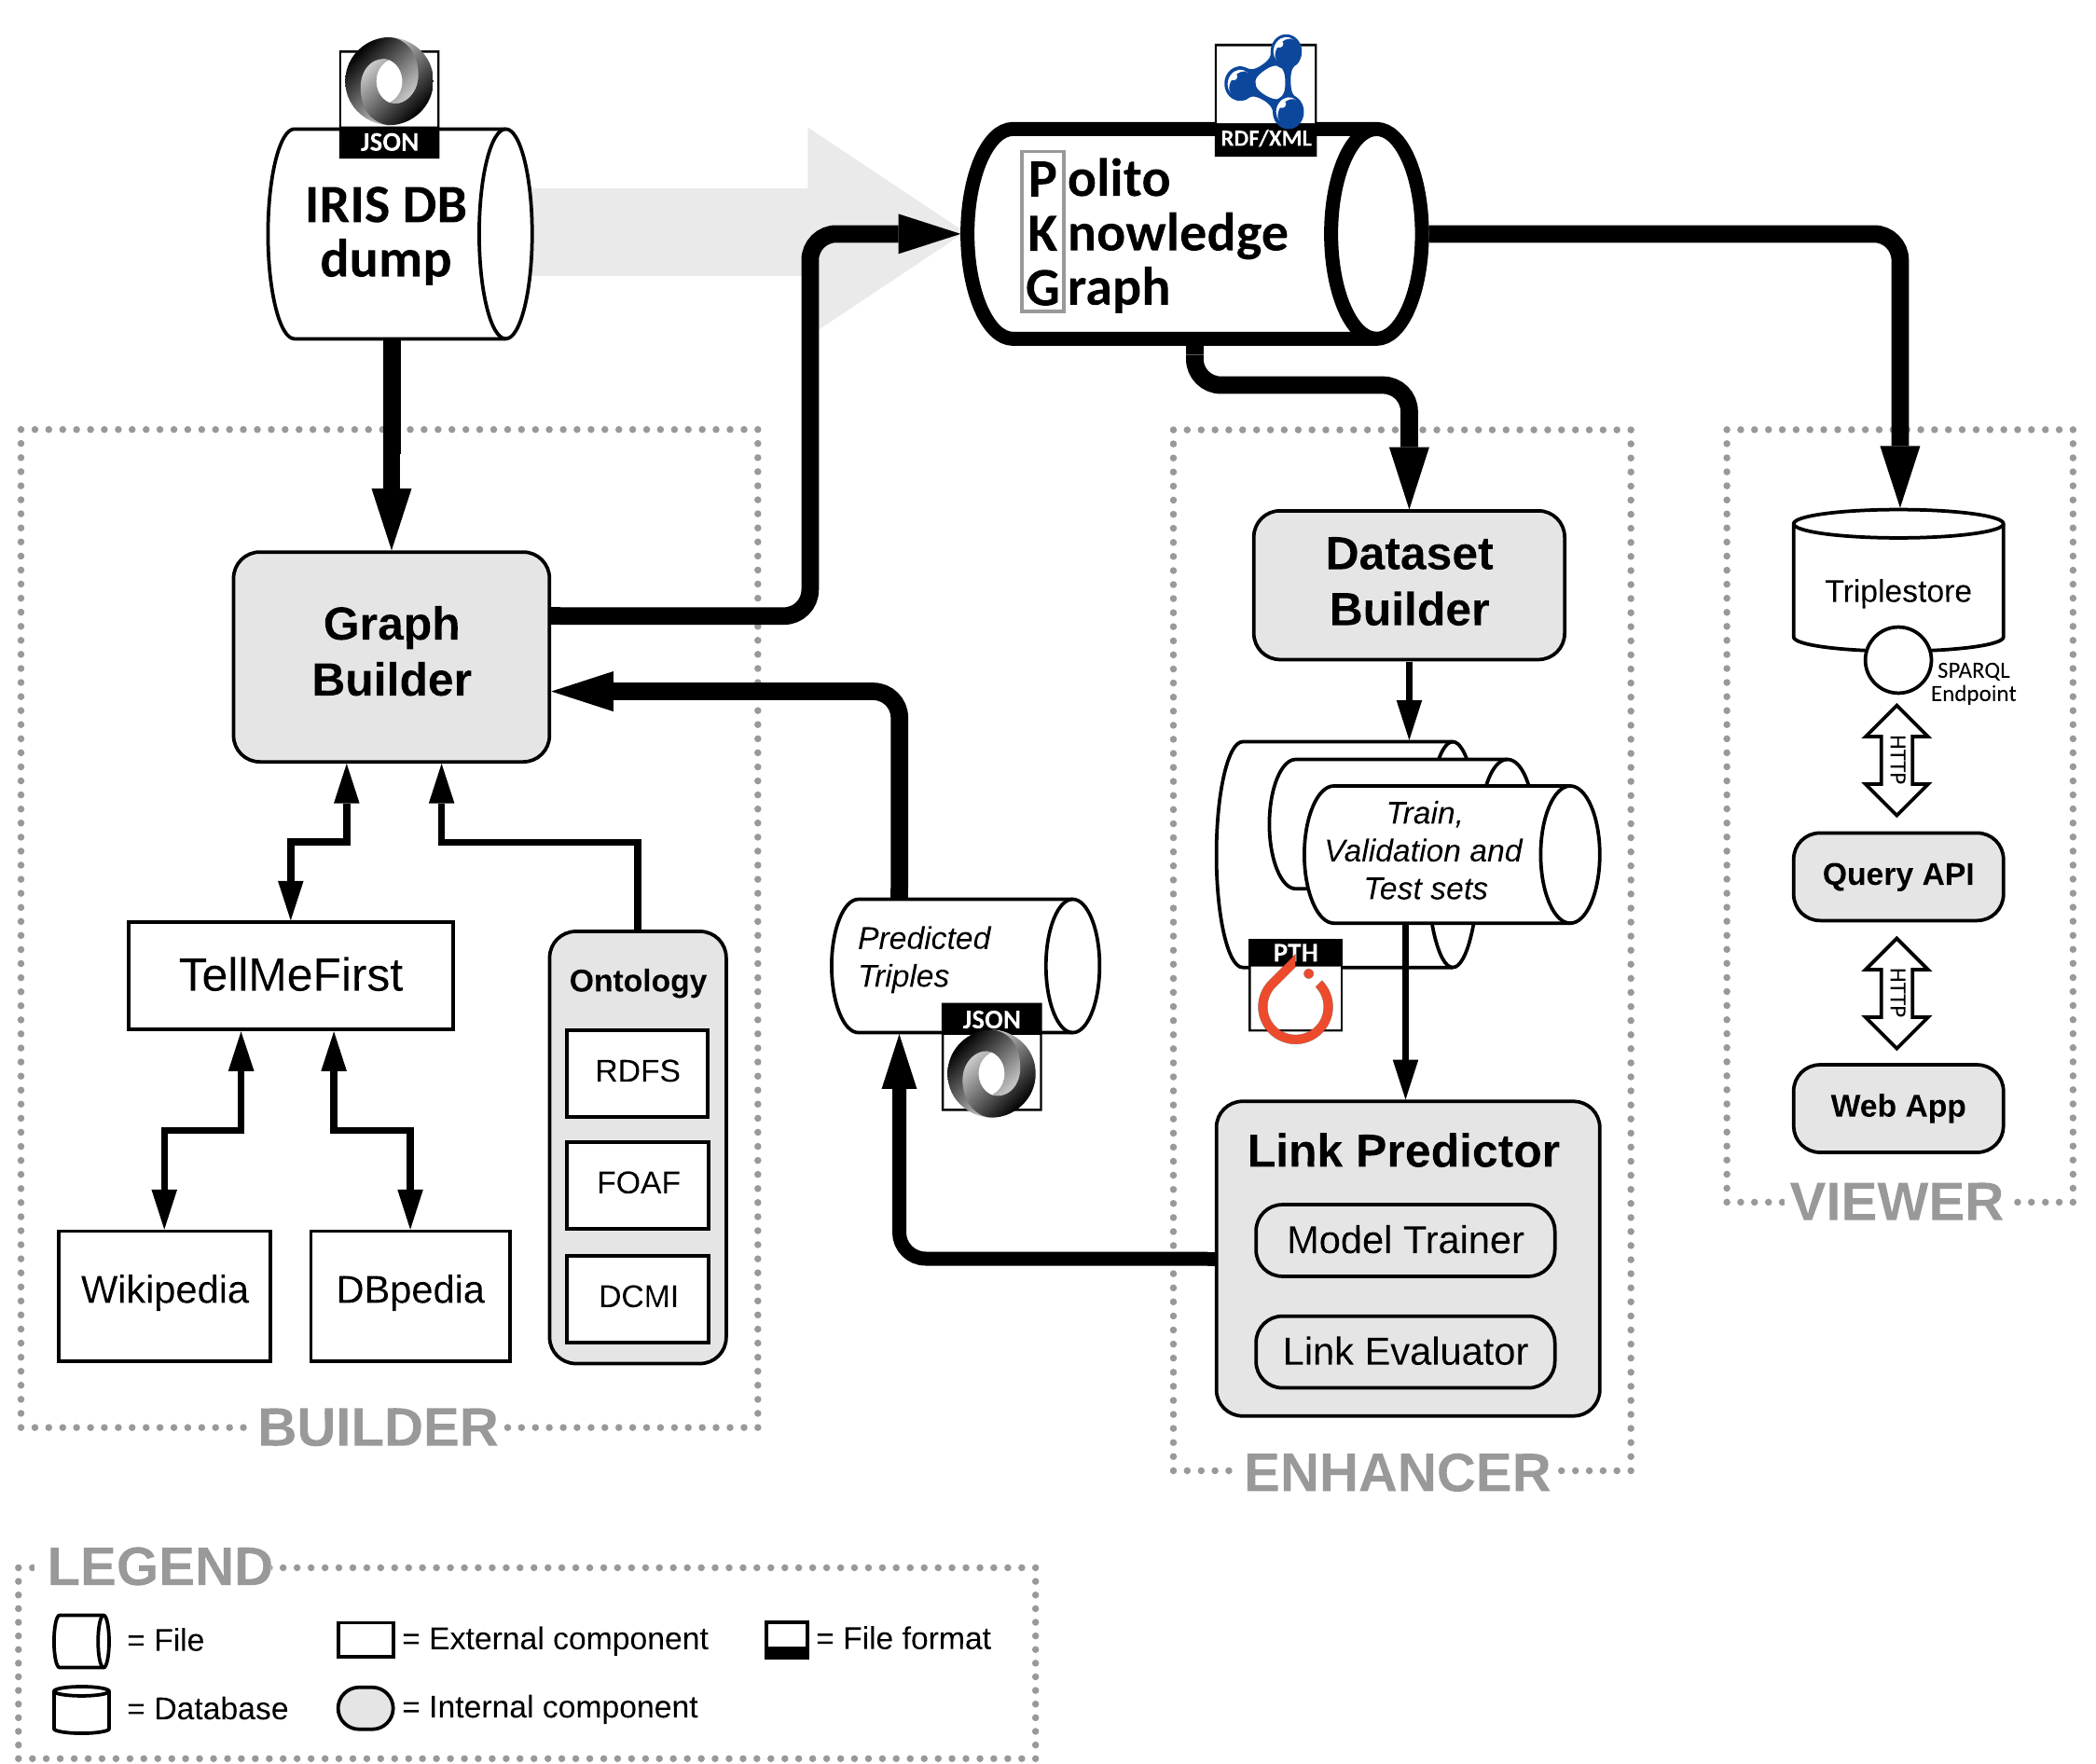
\includegraphics[scale=0.8]{img/pipeline.png}
    \caption{Schema of the pipelined software architecture developed to build,
    enhance and visualize the Polito Knowledge Graph.}
    \label{fig:pipeline}
\end{figure}


\section{Builder Module}

The Builder input is a dump of the
IRIS\footnote{\url{https://iris.polito.it/}} database, which is the platform
used by the Politecnico di Torino to store and share all the
scientific papers written by its researchers. The dump is a
JSON file that contains all the information available for the scientific
paper published in a period of five years that goes from 2013 to 2017.

The Builder goal is to translate all the information contained in the
dump in a set of semantically coherent RDF triples. To do so, an ontology that
describes the domain of the IRIS scholarly data has been defined.

The builder uses as reference the defined ontology to analyze each record in
the JSON dump, and builds facts as RDF triples by matching the information
contained in the record with the concepts defined by the ontology.
For example, given that a publication may have more then one contributor, the
ontology that we defined differentiates the principal author from the
contributors by using two different statements to tie the corresponding entities
to the publication.

One of the fields of the publication record is the abstract. We wanted to
link each publication to its research fields, to do so we used the publication abstract
as input text for TellMeFirst (TMF) \cite{rocha2015}, a tool for the automatic
extraction of semantic keywords from texts. Such keywords, to which from now
on we'll refer to as \emph{topics}, are retrieved from the DBpedia taxonomy
and are uniquely identified by their corresponding URI.
By exploiting TMF we are able to automatically tie each publication to
its relevant topics, by adding the corresponding RDF statements to the graph.
Being the topics added as graph entities which are uniquely identified, all the
publications that share a topic are linked to the same topic entity.

The result of this process is a set of RDF statements that constitutes the
first version of the Polito Knowledge graph, a semantically coherent description
of the publications produced by the Polito researchers, where each
publication is uniquely identified and linked by means of semantic relations
to the entities representing its authors, contributors and research topics.


\section{Enhancer Module}

Once the first version of the RDF graph has been built, it could be used as
input for the Enhancer Module, whose main goal is to infer unseen facts to
complete and enhance the information available inside the knowledge graph.
\newline

The Enhancer is composed of three main components:

\begin{enumerate}
    \item The Dataset Builder.
    \item The Model Trainer.
    \item The Link Evaluator.
\end{enumerate}

The Dataset Builder is in charge of translating the RDF graph into a usable
dataset for the Model Trainer, this because the RDF statements cannot be used as
input data for the link prediction algorithm.
The dataset will then be splitted into three disjoint\footnote{Two sets are said
to be disjoint if they have no element in common.}
sets.

The Model Trainer uses this three sets to train, validate and test the link
prediction model.
The training set is used to train the model at each epoch, while the validation set
is used to evaluate which model parameters to keep, identifying the best epoch.
The test set is used to evaluate the accuracy of the model, loaded with the best
epoch parameters, upon unseen triples. Once the model has been trained, it can
be used to predict unseen facts.

The Link Evaluator loads the best model found during the training phase and
uses it to evaluate unseen triples.
To do so, the Evaluator creates a set of unseen RDF triples and produces a score
for each of them. Only the triples that obtain an high score (and so have an high
probability to be true facts) and are correct in domain and range with respect
to the ontology are kept.
The predicted triples are then saved as RDF statements and could be added
to the RDF graph, obtaining the enhanced version of the Polito Knowledge Graph.
This new version will contain not only the information available on IRIS, but
also the latent information inferred by the learnt model, like missing topics,
similar authors or proposed journals, which can be used to empower a
recommendation system for the Polito researchers.

\section{Viewer Module}

The last module of the architecture is the Viewer, which is composed of a
triplestore, an API layer, and a front end web interface.

The triplestore is a specialized DBMS for storing and retrieving RDF
statements.
It stores an online copy of the Polito Knowledge Graph and expose a
SPARQL endpoint that allows to query the graph itself.

The API layer exposes a REST API that allows to retrieve the information
contained in the graph without the need of using SPARQL queries. It accepts HTTP
requests with URL-encoded parameters and proceeds to query the SPARQL endpoint
of the triplestore by matching the parameters upon some predefined queries.
Then, it translates the response obtained from the triplestore in a JSON file,
which is sended back to the requesting client, which is typically the front end.

The front end is a responsive web application that act as the entry point for
the user, mimicking the functionalities of a modern search engine. It allows
to query and visualize the data contained in the graph through the use
of a simple and friendly User Interface.

For example the user, who should typically be a researcher of the Politecnico di
Torino, can search for a topic of interest and obtain as result the list of all
the publications, authors and journals that are linked to such topic.
The predictions are used to add suggestions to the results, for example,
if searching for an author, in the results obtained are shown not only its
actual research interestes, but also other topics in which he may interested in,
or researchers with similar profiles but with which he never published a
research together, thus obtaining useful insights about its scientific community.




%%%%%%%%%%%%%%%%%%%%%%%%%%%%%%%%%%%%%%%%%%%%%%%%%%%%%%%%%%%%%%%%%%%%%%%%%%%%%%%%
% -------------------------------- Related Work ------------------------------ %
%%%%%%%%%%%%%%%%%%%%%%%%%%%%%%%%%%%%%%%%%%%%%%%%%%%%%%%%%%%%%%%%%%%%%%%%%%%%%%%%
\chapter{Related Work}

% Open Academic Graph
Today there is a growing interest in scientific
knowledge graphs, both from academic institutions and private organizations.
An example is the Open Academic
Graph\footnote{\url{https://www.openacademic.ai/oag/}} (OAC), an academic
knowledge graph that has been built by merging together two of the largest
scientific KG available, the Microsoft Academic
Graph\footnote{\url{https://academic.microsoft.com/}}
and AMiner\footnote{\url{https://www.aminer.cn/}}.
The OAC has been publicly released to allow
the study of citation networks, papers content and more.
The first version of the graph, released in 2017, has been
built by merging together the aforementioned graphs and by linking the
matching publications, obtaining a graph that is composed of more then three
hundred million publications. In the first version of the graph the only kind of
entity present was the publication: authors, journals, and all
the other publications metadata were added as attributes, and not as entities.

In January 2019 the second version of the Open Academic Graph has been
released, adding even more publications to the graph.
However, the biggest change of this new
version was the addition of authors and venues as graph entities,
instead of being simple publications attributes.

However, the OAC does not contain the publications topics as graph
entities, but as author keywords, thus being prone to the same limitations of
IRIS: the keywords are the ones chosen by the authors and are not
referencing to semantic concepts, being simple character strings.
\newline

% wiser
Regarding the development of tools similar to the Polito Knowledge Graph
by other academic institutions, an example of employment of knowledge graphs
and natural language processing techniques to build new academic search engines
is Wiser\cite{cifariello2019}, an
expertise search tool developed by the University of Pisa and publicly released
at the beginning of 2019.
The knowledge graph of Wiser is composed of approximately 1'500 authors, 65'000 publications
and 35'000 topics\footnote{Details about the Polito Knowledge Graph dimensionality and scale
will be presented in the following chapter.}.
The system has proven to be particularly effective, representing a strategic
tool and being actively used by the university Technological Transfer Office to
easily find expertise profiles in a given research field.
\newline

% CSO Classifier and Computer Science Ontology
As saw in the previous Chapter, one of the main components of the PKG
pipeline is TellMeFirst, tool used to automatically extract the topics of
interest from the publications abstracts. By automatically extracting the
topics, TMF allows to add them as entities in the Polito Knowledge Graph,
so that each publication is directly linked to its main topics, and each topic
is linked to all the publications of which it is a subject (reverse relation).

Other tools that are able to extract the subjects of a publication exists, an
example is the CSO Classifier \cite{salatino2019}. This tool is able to
automatically classify a research paper according to the Computer Science
Ontology\footnote{\url{https://cso.kmi.open.ac.uk/home}} (CSO), an automatically
generated ontology of research topics in computer science.
The fact that the CSO Classifier relies on a predefined ontology has some
disadvantages with respect to TellMeFirst, the biggest being the fact that the
Computer Science Ontology is restricted to the computer science field only,
while TMF, using DBpedia as its source of knowledge, is able to extract
topics (and so to classify a research paper) regarding every field of research.
However, the approach of CSO Classifier has also its advantages: being the
ontology more restricted, the classification could be more accurate, and the
structure of the ontology itself may be tailorized for such classification task.

% R-GCN
Regarding the learning task on graph data, many architectures that implements
the Message Passing Framework\cite{gilmer2017} and that are derived from the
classical Convolutional Neural Network are available, some example being
\cite{defferrard2016} and \cite{duvenaud2015}.
We decided to implement the R-GCN architecture for our prediction task
being specifically designed to work with relational graph data.
Moreover, due to the different approach followed by the authors of R-GCN, which
relyies on the convolutional architecture only as an encoder, in future works
we could try different factorization methods while keeping the same encoder
architecture based on R-GCN to learn the node embeddings.
Some possible factorization methods that we would like to implement
as decoders are \cite{kazemi2018} and \cite{trouillon2016}.
However, to the best of our knowledge, we are the first to leverage a
Relational-GCN for the completion task of an academic knowledge graph.




%%%%%%%%%%%%%%%%%%%%%%%%%%%%%%%%%%%%%%%%%%%%%%%%%%%%%%%%%%%%%%%%%%%%%%%%%%%%%%%%
% ----------------------- Development and Implementation --------------------- %
%%%%%%%%%%%%%%%%%%%%%%%%%%%%%%%%%%%%%%%%%%%%%%%%%%%%%%%%%%%%%%%%%%%%%%%%%%%%%%%%
\chapter{Development and Implementation}

In the first part of this chapter we will describe the development and the
implementation of the Polito Knowledge Graph, particularly focusing
on the components in charge of the graph creation and enhancement, whose
architecture has been introduced in Chapter \ref{ch:approach}.

We will firstly introduce a detailed description of the input data used to
create the graph. We will also describe the ontology used to shape the
knowledge of the scholarly domain and the graph schema obtained by structuring
the information made available by IRIS with such ontology.
Then, we will discuss how we implemented the Builder Module, which is
responsible for the actual creation of the Polito Knowledge Graph starting
from the IRIS publications metadata.

In the second part of the chapter we will focus on the implementation of the
link predictor module, which is used to predict new facts inside the knowledge
base.
We will describe how we created a usable dataset for the training of an
encoder model starting from the Polito Knowledge Graph, which
architecture and hyperparameters we choose, how we trained such model and
how it has been validated during the training phase in order to choose the
best parameters.
We will also discuss how we tested the model and which metrics we chosen
to evaluate the accuracy of the predictions on the test set.

Finally, we will present how we employed the trained model to obtain
predictions about new facts, and how the predictions obtained
can be used to build a recommendation system for the Polito Knowledge Graph.


\section{Building the Polito Knowledge Graph}
\label{sec:buildingpkg}

As already mentioned when introducing the pipeline in Chapter \ref{ch:approach},
the input data used to
build the PKG is a dump of the IRIS database, which contains the information about
the scientific papers published by the researchers of the Politecnico di
Torino in a five-year period.
The dump is a JSON file composed of 23,268 records, and each record contains
the metadata of a single scientific publication.
Many of the available metadata are generated by the IRIS platform, in
order to manage its internal processes of publications management.
We have discarded such information, since they are not
significant for the publication characterization.

We selected the following metadata as the ones that truly characterize a
scientific paper:

\begin{enumerate}
    \item The publication identifier.
    \item The title.
    \item The abstract.
    \item The author name, surname and identifier.
    \item The contributors and coauthors names, surnames, and identifiers
        (if present).
    \item The date of publication.
    \item The journal title and ISSN (if present).
    \item The keywords entered by the authors to tag the publication.
\end{enumerate}

The publication identifier is a unique numeric code associated by IRIS to each
scientific paper. Also the authors, contributors and coauthors should be
uniquely identified by an alphanumeric identifier, however, only the researchers
of the Politecnico di Torino have such identifier. External
researchers that may be contributors or coauthors of the publication are present
with only their name and surname.
The author is instead always a Polito researcher.

If the scientific paper has been published in a journal, the journal ISSN
is used as identifier, if present.
If the publication is a conference paper, no information about the conference
is present other than the title, thus we cannot uniquely identify the
conference, at least in this first version of the Graph Builder.
The publication title, the abstract, the names, surnames and the keywords and
the date of publication are simple character strings.

As already discussed in previous Chapters, the keywords entered by the authors
cannot be treated as semantic concepts. We wanted to solve this issue, in order
to have all the publications that refer to a specific topic linked to a
same semantically unambiguous graph entity that uniquely represents such topic.
To do so, as already mentioned in the previous Chapter, we employed
TellMeFirst (TMF), a tool for the automatic extraction of
semantic keywords that relies on the DBpedia ontology and knowledge graph as
its source of knowledge.

In the following sections we will describe how we developed the Graph Builder
and how, leveraging TMF, we have been able to extract the relevant topics of a
publication from its abstract, adding such topics as graph
entities in the Polito Knowledge Graph.

\subsection{PKG Ontology and Schema}

Starting from the metadata discussed above, we defined
the PKG ontology as composed of five different classes:

\begin{enumerate}
    \item The \emph{Publication}.
    \item The \emph{Author}.
    \item The \emph{Journal}.
    \item The \emph{AuthorKeyword}.
    \item The \emph{TMFResource}.
\end{enumerate}

In order to build a knowledge graph, the instances of such classes must be
linked together by means of semantic relations, called predicates.
To do so, we employed some predicates already defined by the
FOAF\cite{brickley2007} and the DCMI\cite{weibel1998} ontologies, together with
some terms defined by the RDFS\cite{lassila1998} standard.
The graph structure obtained is represented by the schema in
Figure \ref{fig:schema}, where we show the classes, the attributes of such
classes and the predicates that links them together.

\begin{figure}[h]
    \centering
    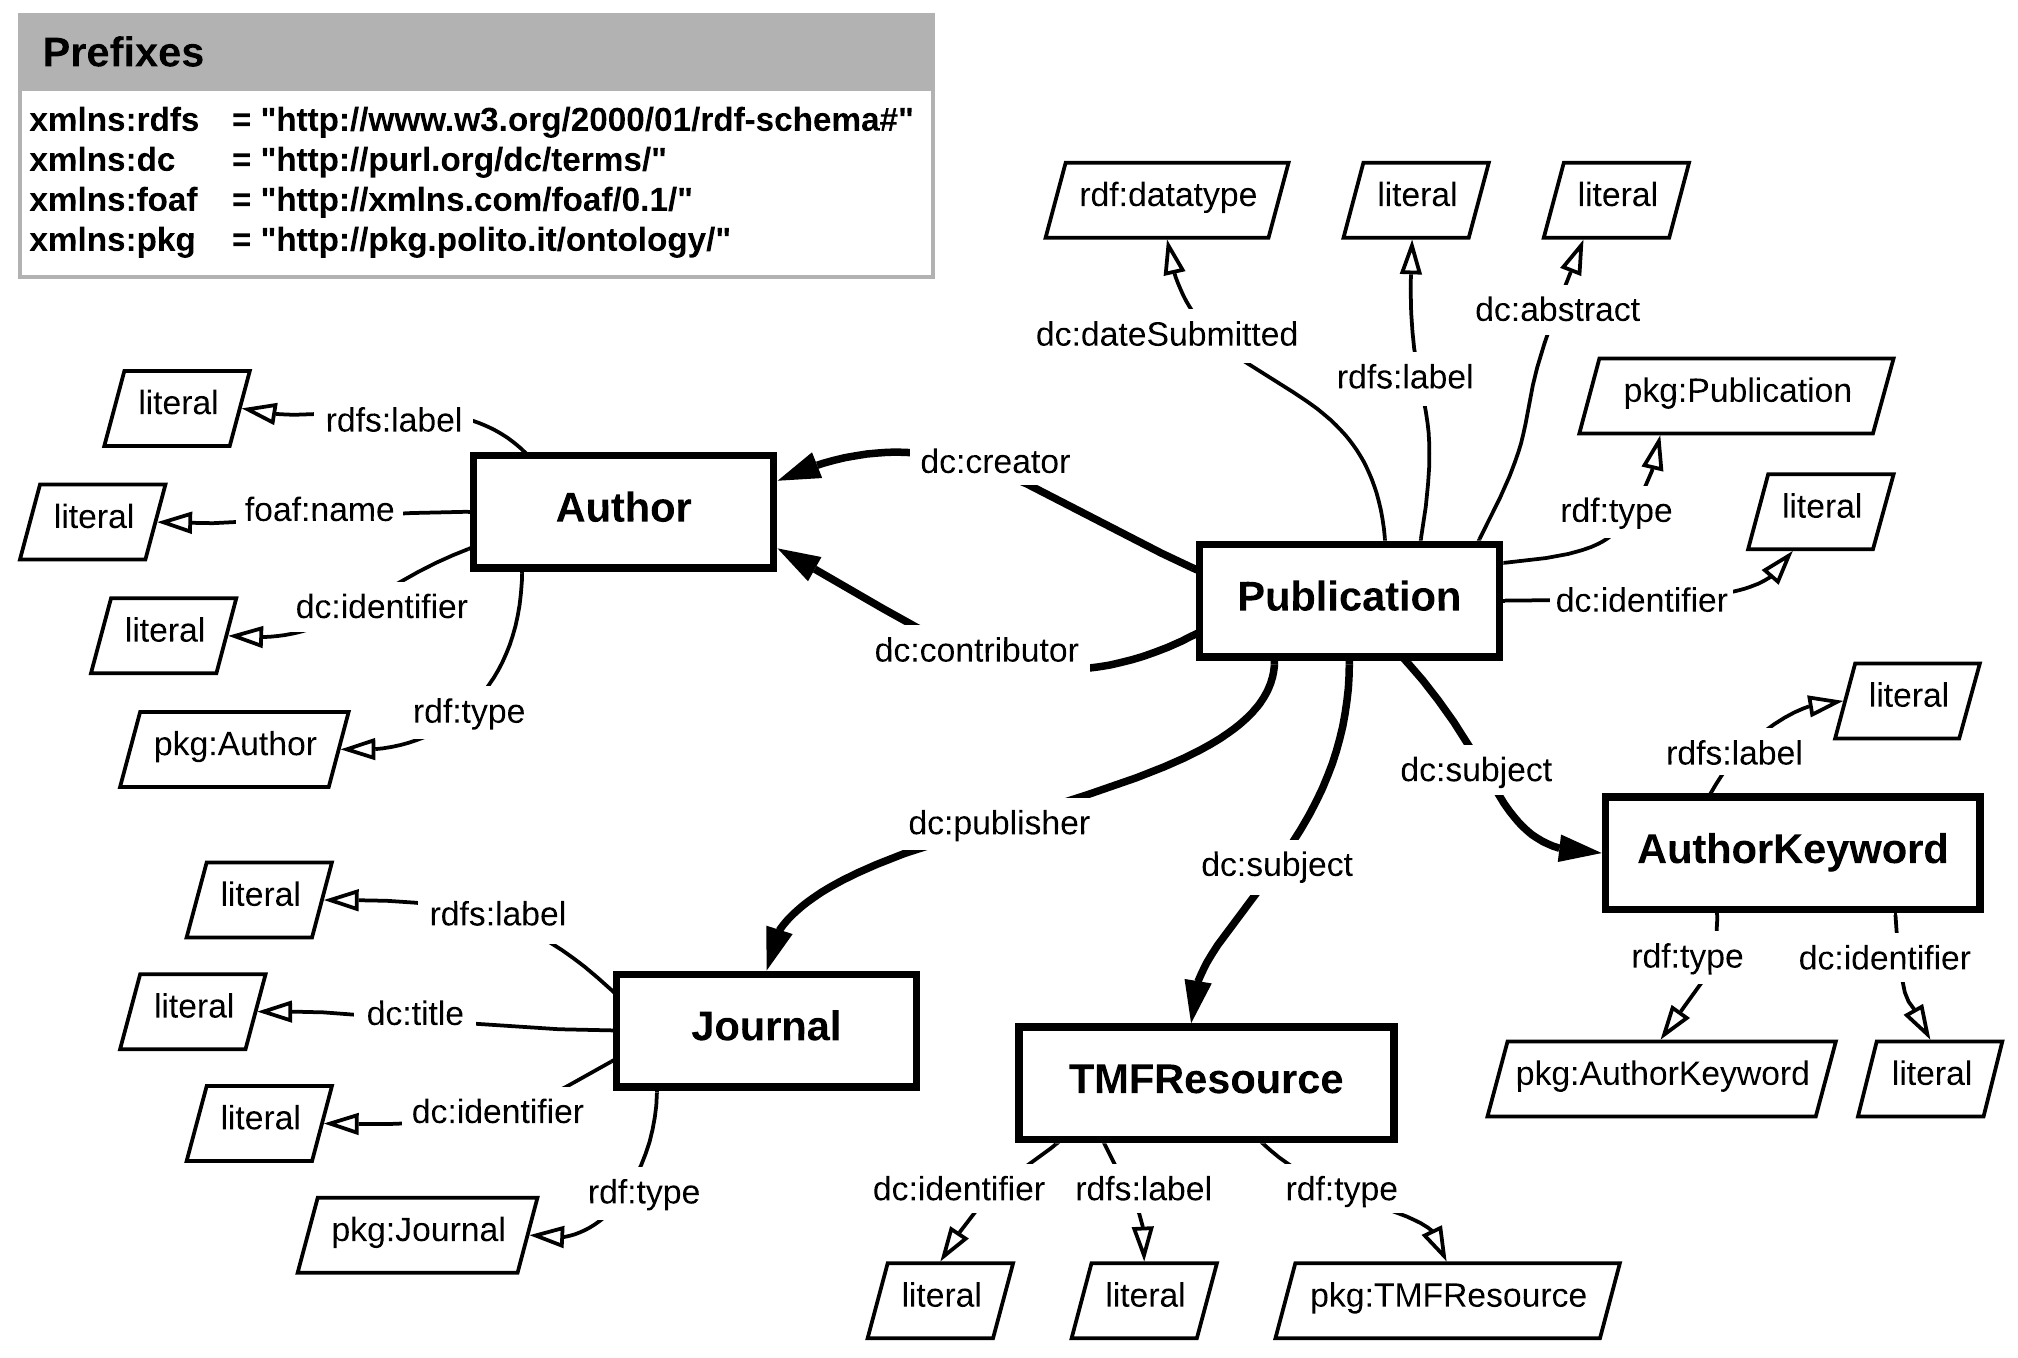
\includegraphics[scale=0.85]{img/schema.png}
    \caption{Schema of the Polito Knowledge Graph. The ontologies used to
    define the structure are shown in the prefixes table.}
    \label{fig:schema}
\end{figure}

As can be saw from the schema shown in Figure \ref{fig:schema}, the
\emph{Publication} class is linked to the \emph{Author} class by means of two
relations both defined by the DCMI ontology:
\emph{dc:creator}\footnotemark and \emph{dc:contributor}\footnotemark[\value{footnote}].
\footnotetext{The \emph{dc} keyword is used as prefix for the Dublin Core
Metadata Initiative (DCMI) namespace: http://purl.org/dc/terms/}

We decided to only differentiate the first author (\emph{creator}) from
the others (\emph{contributors}) due to the inability to discriminate, based
on the metadata made available by IRIS, which are
the co-authors and which are the collaborators.

The \emph{AuthorKeyword} class represents the keywords added by the authors
to tag the publication.
Even if such keywords do not represent any semantic information, we decided to
add them to the knowledge base for the sake of completeness with respect to
the metadata available.

Instead, the \emph{TMFResource} class is used to categorize the entities
corresponding to the DBpedia resources extracted by TMF starting from the
publications abstracts.
Being uniquely identified by their DBpedia URI, the publications that shares
a topic will be linked, through the \emph{dc:subject} relation, to the same
instance of the \emph{TMFResource} class that represents such topic.
An example is shown in Figure \ref{fig:subject-knowledge-base}, where are
depicted all the publications that are linked to the entity instantiated for
the \emph{Knowledge Base} topic.

\begin{figure}[h]
    \setlength{\belowcaptionskip}{-25pt}
    \centering
    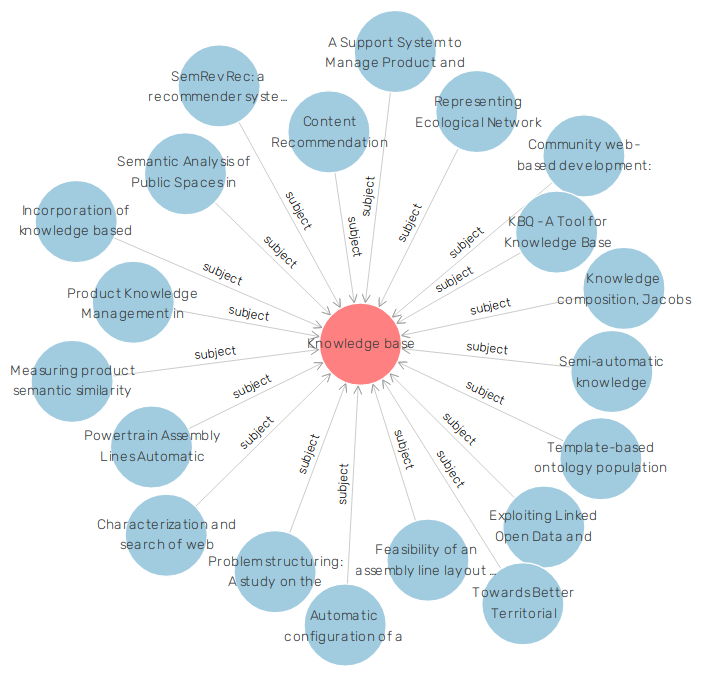
\includegraphics[scale=0.35]{img/subject_knowledge_base.png}
    \caption{
        Visualization of the results obtained from
        the PKG when running a SPARQL query that returns
        all the publications that have \emph{Knowledge Base}
        as topic.
        An excerpt of the RDF representation of this example will be listed in
        the following section.
    }
    \label{fig:subject-knowledge-base}
\end{figure}



\subsection{The Graph Builder}

We implemented the Graph Builder as a Python command-line script that uses
the \emph{rdflib}\footnote{\url{https://github.com/RDFLib/rdflib}} library
to create and manage an in-memory RDF representation of the graph.
Such representation can be then serialized and saved as an XML file.
The script takes as arguments the path to the JSON dump of IRIS, together
with some options that allows to trigger specific functionalities of the
script, such as:

\begin{enumerate}
    \item The update of an already existing RDF graph with new statements,
        used for example to add the predicted triples.
    \item The number of topics that must be extracted from each abstract by
        TMF, the default value is seven.
    \item The addition of the URLs of
        the topics pictures, which are scraped from Wikimedia
        Commons\footnote{\url{https://commons.wikimedia.org/}} through
        its publicly available SPARQL endpoint and added
        to the corresponding \emph{TMFResource} instances.
\end{enumerate}

The Graph Builder firstly declares the namespaces and the ontology used to
define the RDF representation of the entities and the relation inside the graph
as written in the previous section, then parses the arguments and options
received and execute the corresponding activities.

If the creation of a new graph is requested, the script reads the JSON dump
in a Python list and instantiates a \emph{ThreadPoolExecutor}, a Python
abstraction that allows to execute a function asynchronously by spawning
a predefined number of threads.
Each thread asynchronously executes a function that process a single record of
the dump.
The concurrent access to the records list is not a problem, being the Python
lists implemented as thread safe containers.
Each record is processed by:

\begin{enumerate}
    \item Matching the record metadata with the ontology classes and
        instantiating the corresponding entities.
    \item Requesting to TMF, via its API, the extraction of the topics
        from the publication abstract.
\end{enumerate}

In the first step, when a field that matches a class is found, a corresponding
RDF triple that instantiates a new object is created, so a new entity is added
to the graph. If the entity is already present, an RDF triple that connects the
publication to the already existing entity is added.

The topic extraction is performed by TMF by sending an HTTP POST request
containing the publication abstract and the requested number of topics to be extracted.
The response contains the list of the DBpedia resources that TMF
extracted as main topics for the publication. Such topics are added to the
graph as \emph{TMFResource} entities, and are
linked to the publication by means of the \emph{dc:subject} relation.

Even if the Python interpreter implementation poses some limitations in the
actual advantage of executing multithreaded code in CPU bound scenarios, in our
case the use of multiple threads  improved the time required to build
the graph, being the implementation I/O bound by the communication with the
REST API of TMF.

The two steps described above allows to generate the RDF description of a
publication starting from its metadata, which is then enriched by the topics
extracted by TMF.
For instance, the listing that follows contains an example RDF description
generated by the Graph Builder. As can be saw, not only a new
publication entity is created, but also the author and the extracted topic are
added to the graph and linked to the publication.

\begin{lstlisting}[
    language=XML,
    frame=single,
    basicstyle=\ttfamily\footnotesize,breaklines=true\small,
    numbers=left,
    backgroundcolor=\color{codebackground}
]
<rdf:RDF
    xmlns:pkg="http://pkg.polito.it/"
    xmlns:dc="http://purl.org/dc/terms/"
    xmlns:foaf="http://xmlns.com/foaf/0.1/"
    xmlns:rdf="http://www.w3.org/1999/02/22-rdf-syntax-ns#"
    xmlns:rdfs="http://www.w3.org/2000/01/rdf-schema#"
    xmlns:dbpr="http://dbpedia.org/resource/"
    xmlns:xmls="http://www.w3.org/2001/XMLSchema#">
    <rdf:Description rdf:about="pkg:publications/2670709">
        <rdf:type rdf:resource="pkg:ontology/Publication"/>
        <dc:identifier>2679709</ns1:identifier>
        <rdfs:label>Title</rdfs:label>
        <dc:abstract>Abstract of the publication</ns1:abstract>
        <dc:subject rdf:resource="dbpr:Knowledge_Base"/>
        <dc:creator rdf:resource="pkg:authors/rp00000"/>
        <dc:dateSubmitted rdf:datatype="xmls:date">
            2017-01-01
        </dc:dateSubmitted>
    </rdf:Description>
    <rdf:Description rdf:about="dbpr:Knowledge_Base">
        <rdf:type rdf:resource="pkg:ontology/TMFResource"/>
        <dc:identifier>Knowledge_Base</dc:identifier>
        <rdfs:label>Knowledge Base</rdfs:label>
    </rdf:Description>
    <rdf:Description rdf:about="pkg:authors/rp00000">
        <rdf:type rdf:resource="pkg:ontology/Author"/>
        <foaf:name>Surname, Name</foaf:name>
        <dc:identifier>rp00000</dc:identifier>
        <rdfs:label>Surname, Name</rdfs:label>
    </rdf:Description>
</rdf:RDF>
\end{lstlisting}

By translating every record of the IRIS database dump into a set of
RDF statements we created an RDF graph composed of entities that are uniquely
identified and linked together by meaningful relations, thus obtaining a
comprehensive representation of the Politecnico di Torino academic community.
The Polito Knowledge Graph links together researchers, their fields of
interest, the scientific papers produced by them and the journals in which
such papers have been published.

% table: Polito Knowledge Graph characteristics
\begin{table}[t]
    \footnotesize
    \centering
    \caption{Number of entities and edges in the Polito Knowledge Graph.}
    \label{tab:pkgsize}

    \begin{tabularx}{1.0\textwidth}{ Y Y Y Y Y }
            \toprule
            \multicolumn{5}{c}{\textbf{Polito Knowledge Graph}} \\
            \midrule

            \addlinespace[0.1cm]
            \multicolumn{5}{c}{\textbf{Number of entities per-class}} \\
            \addlinespace[0.2cm]
            Publication & Author & Journal & TMFResource & AuthorKeyword \\
            23,268 & 34,886 & 3,211 & 16,988 & 41,807 \\
            \midrule

            \addlinespace[0.1cm]
            \multicolumn{5}{c}{\textbf{Number of edges per-relation}} \\
            \addlinespace[0.2cm]
            Creator & Contributor & Publisher & Subject (TMF) & Subject (Keywords) \\
            23,268 & 80,819 & 11,243 & 107,093 & 77,492 \\

            \bottomrule
    \end{tabularx}
\end{table}

In Table \ref{tab:pkgsize} we summarized some statistics about the size of the
PKG, showing the number of entities instantiated for each class, and the
number of edges for each relation type.

After all the publications have been processed by the Graph Builder, the
internal representation of \emph{rdflib} can be serialized and exported as an XML
file that contains the definition of all the RDF triples that forms the
Polito Knowledge Graph.
Such RDF representation can be then used as input for the Enhancer Module or
loaded into a triplestore (for example
Blazegraph\footnote{\url{https://blazegraph.com/}}) in order to be queried by
the viewer component.
\newpage




\section{Enhancing the Polito Knowledge Graph}

Once the first version of the Polito Knowledge Graph has been built, the
Enhancer Module can be used toe inference new facts. In this Chapter is
presented how, starting from the RDF graph, we created a usable dataset
for the link predictor, how we employed a R-GCN architecture to encode the
entity characteristics into meaningful embeddings and how we obtained and
evaluated the predicted triples.


\subsection{The Dataset Builder}

The Model Trainer can not learn the nodes embeddings by directly taking as input
the RDF representation of the graph.
To solve this issue, another component, the Dataset Builder, is in charge of
creating a useful dataset for the learning task.

As discussed in the previous Chapter, some of the metadata available
in the IRIS publications records are not uniquely identified, however, we
have still added them to the graph for the sake of completeness.
As a consequence of this, the corresponding entities do not represent
unhambiguous semantic information, the effect being that such entities may
only add noise to the dataset, thus leading to incorrect predictions.

To avoid this issue, we decided to include in the dataset only the entities
which are unique and unhambiguous in the whole graph:

\begin{enumerate}
    \item The publications, identified by their IRIS ID.
    \item The authors, identified by their Politecnico di
        Torino internal ID.
    \item The journals, identified by their ISSN.
    \item The topics extracted by TMF, identified by their DBpedia
        URI.
\end{enumerate}

With respect to the full set of entities of the Polito Knowledge Graph, we
discarded all the external contributors and co-authors, for which we only have
as information the names and surnames, and all the authors keywords.
The dataset is thus built from a reduced version of the initial graph.

In the following, we will explain how starting from such reduced version of the
graph we built a usable dataset for the learning task.
\newline

Like the Graph Builder, also the Dataset Builder is implemented as a
Python command-line script that process the RDF graph triples with \emph{rdflib},
which offers a practical interface to work with RDF data.
The Dataset Builder has to convert the RDF representation of the graph into
an integer representation, where each class, entity and relation has a
corresponding integer index assigned.

The following input data are needed by the Model Trainer to train the
encoder:

\begin{enumerate}
    \item The number of nodes, equal to the number of entities instantiated by
        the RDF statements.
    \item The number of different relations that links together the graph
        entities.
    \item The number of nodes labels, where each label is referred to a class of
        the PKG ontology.
    \item A list of edges, where each edge is a Python tuple composed of three
        elements: the node index of the subject and the object, and the
        index of the predicate. How such indexes are generated is
        explained in the following.
    \item A list of node-specific normalization constants.
\end{enumerate}

To build such data structures starting from the RDF graph, the Dataset Builder
leverages some look-up hash tables (implemented as Python dictionaries) that are
created starting from the RDF statements and the PKG ontology. Such tables
are accessed by URI, and allow to retrieve the corresponding entity or
relation integer index.

\begin{enumerate}
    \item The \emph{nodes table} is populated by assigning to each entity
    a unique, increasing integer index. Such index will identify the entity when
    building the list of edges. Only the entities that are instances of the
    classes that we selected as part of the dataset are added to the table.

    \item The \emph{relations table} is built starting from the PKG ontology,
    assigning to each relation inside the graph a corresponding integer
    identifier.
\end{enumerate}

When building such tables, the Dataset Builder also keeps track of the total
number of nodes and relations, and builds a labels list that stores in the
$i$-th element the class (label) of the $i$-th node.

Once the look-up tables and the other data structures are built, the Dataset
Builder starts to process the RDF statements that composes the graph by
looping through them.

\begin{figure}[h]
    \centering
    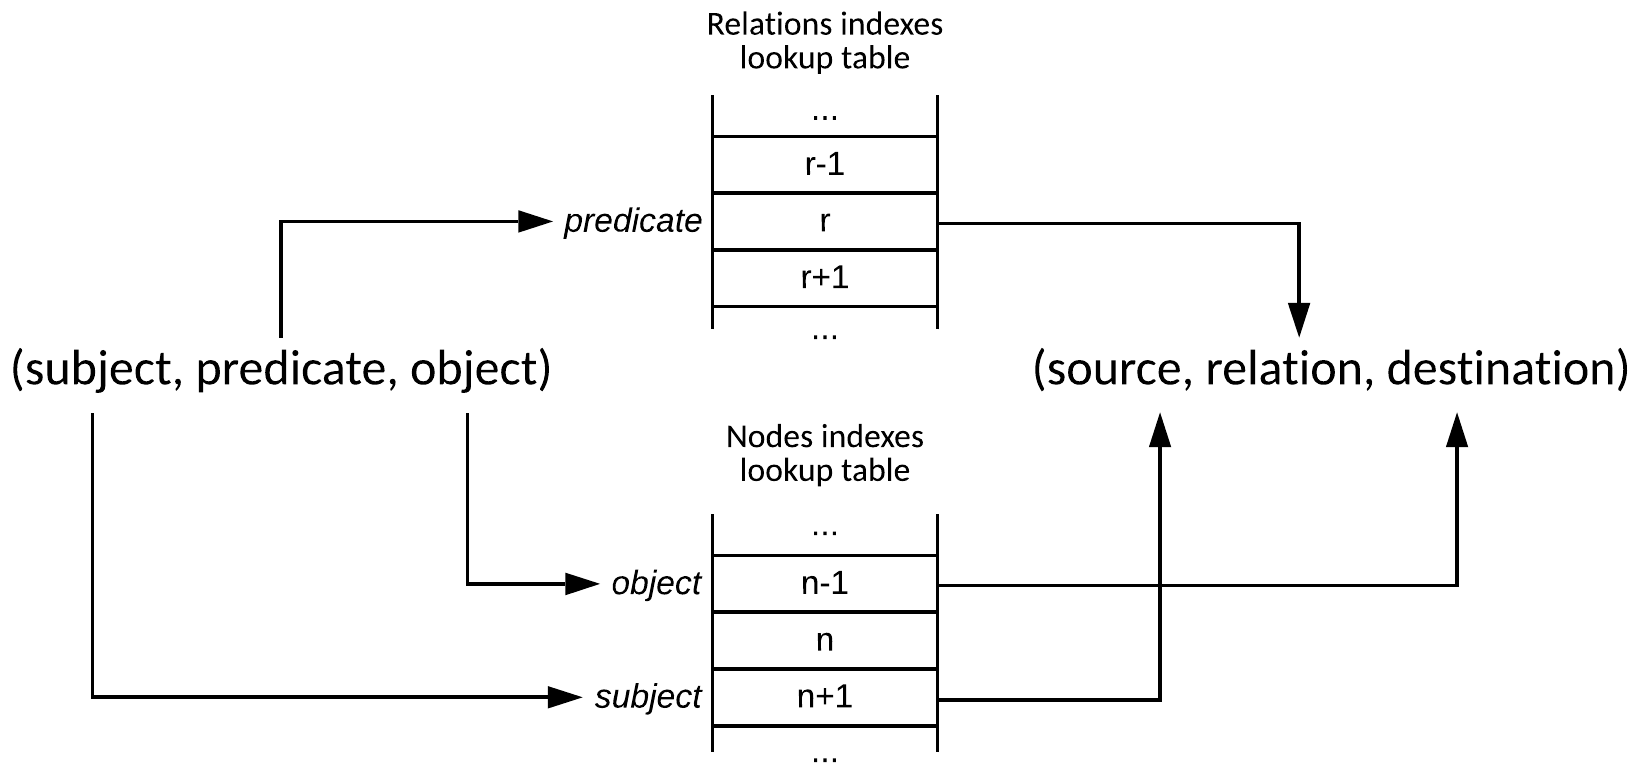
\includegraphics[scale=1.0]{img/rdftodata.png}
    \caption{
        Process of translation from RDF statement composed of URIs to edge
        tuple composed of integer indexes.
    }
    \label{fig:rdftodata}
\end{figure}

For each statement, The Dataset Builder firstly checks wether the subject and
object of the statement are present in the nodes table, if so, it builds the
corresponding edge tuple by retrieving the indexes of the entities and relation
through the look-up table.
An example of this process is shown in Figure \ref{fig:rdftodata}.

The obtained list of edges is then splitted into three separate and disjoint
sets that will be used to train, evaluate and test the encoder model, making
sure to have in the training set, for each node, at least one edge for
every kind of relation present in its directly connected edges.
This is mandatory to obtain meaningful embeddings, because
as already explained in section \ref{subsec:linkprediction}, the R-GCN model
learns the vector representations of the nodes by embeddings the nodes neighbors
features. As a consequence of it, is crucial to have a neighborhood structure
in the training graph which is similar to the one in the full graph.
Once such initial sampling has been done, the remaining training edges are
randomly taken.

The percentage of tuples used to create the three sets is an
hyperparameter that can be choosen in advance. However, during our tests, we
experienced that picking less then 70\% of nodes for training does not allowed
us to maintain a representative neighborhood for each node, resulting in an
inaccurate link prediction model.
To solve this issue, we decided to split the edges list in
approximately 90\% of the tuples for train, 5\% for the validation and 5\% for
testing.

Once the dataset have been created and the list of edges splitted into the three
sets, it is serialized and saved, so that for future run of the Model Trainer
is not required to create the dataset from scratch.
Moreover, since a part of the edges are randomly picked, this allowed us to
evaluate the different hyperparameters values upon the same set of triples.

% table: Polito Knowledge Graph characteristics
\begin{table}[t]
    \footnotesize
    \centering
    \caption{Statistics of the dataset produced by the Dataset Builder.}
    \label{tab:datasetsize}

    \begin{tabularx}{1.0\textwidth}{ Y Y Y Y }
            \toprule
            \multicolumn{4}{c}{\textbf{Dataset}} \\
            \midrule

            \addlinespace[0.2cm]
            Number of nodes & Number of classes/labels & Number of relations & Total number of edges \\
            \addlinespace[0.1cm]
            47,996 & 4 & 4 &  170,593 \\
            \addlinespace[0.2cm]

            \bottomrule
    \end{tabularx}

    \begin{tabularx}{1.0\textwidth}{ Y Y Y }
        \addlinespace[0.2cm]
        \multicolumn{3}{c}{\textbf{Number of train, evaluation and test samples}} \\
        \addlinespace[0.2cm]

        Train edges & Evaluation edges & Test edges \\
        153,531 & 8,528 & 8,534 \\

        \bottomrule
    \end{tabularx}


\end{table}

Table \ref{tab:datasetsize} summarizes the characteristics of the
dataset obtained by the Dataset Builder.
The size of the dataset, in particular the number of nodes and edges,
can be compared to the size of the initial RDF graph, whose statistics are
available in Table \ref{tab:pkgsize}.
As can be saw, more then half the nodes, the ones referred to the
author keywords and the external authors, have been removed.


\subsection{The Model Trainer}

Modern machine learning algorithms are implemented as deep networks
composed by many layers and parameters. Building such architectures from the
ground-up would be almost unfeasible, especially when dealing with challenging
kinds of data structures, such as multi-relational graphs.
Many frameworks and libraries that allow the implementation of complex
architectures without the need of coding them from scratch. Moreover, one
of the key aspects when coding machine learning models is to build highly
efficient implementations, especially when working with giant data structures,
as in the case of knowledge graphs, thus leveraging highly optimized and tested
software is crucial.

% pytorch
One of the most common used frameworks that allows to build and train
ML models is PyTorch \cite{paszke2017}. The goal of PyTorch is to provide
some simple yet expressively powerful components that could be used to implement
any sort of neural network, simplifing some of the most challenging aspects,
like the implementation of the backpropagation phase.
The two major abstractions introduced in the framework are the \emph{tensor}
and the \emph{autograd}.
Tensors are the basic data structure in PyTorch, they support both CPU and GPU
execution and all the major operations for multidimensional matrices.
The autograd package is the key novelty of PyTorch, allowing to perform
automatic differentiation of all the operations performed on tensors by
leveraging an internal representation in the form of a computational graph.
However, even if PyTorch provides all the building blocks for
developing complex neural networks, it is not suitable when dealing with graph
data due to the lack of support for the message passing paradigm (which has been
introduced in Chapter \ref{sec:learninggraphs}) by the
tensor interface.

% dgl
Deep Graph Library \cite{wang2019} (DGL) provides a more comprehensive
solution specifically designed to work with graph data. DGL is built on top of
existing ML frameworks (e.g. PyTorch, MXNet), and offers a simple
interface that facilitate the implementation of the message passing framework.
Supporting such framework, with DGL is possible to implement every deep learning
algorithm whose forward pass can be divided into a per-edge message computation
and a per-node message aggregation.
Some of the architectures that can be implemented
are depicted in \cite{gilmer2017}, with R-GCN being one of them.

With DGL, a graph can be created by instantiating an object of the
\emph{DGLGraph} class, which offers a dictionary-like interface for adding to
the graph both nodes and edges, together with their features or any other
relevant data for the training, for instance the normalization constants.
The message passing paradigm is implemented by means of the \emph{send} and
\emph{recv} functions, which allows to define the two basic operations for the
per-edge messages construction and the per-node aggregation.

As already mentioned before, we decided to use a R-GCN architecture to build
an encoder model which is capable to produce the nodes embeddings starting
from the graph structure.
Later in this Chapter is discussed how the encoder model has been trained, how
it has been implemented with DGL, which learning problem the model had
to solve and how it has been evaluated, so to chose the best parameters for the
learning task.
\newline

% hardware used
To train and test the model we used a workstation whose hardware and software
specifications are summarized in Table \ref{tab:workstation}.
The same worskation have been used to execute both the Model Trainer and
the Link Evaluator components.
As we will discuss later, the training and evaluation speed have been
bottlenecked by the single core performance of the CPU and by the GPU
memory at our disposal.

% table: Workstation specifications
\begin{table}[h]
    \footnotesize
    \centering
    \caption{Hardware and software specifications of the workstation used to
        run the Model Trainer and the Link Evaluator.}
    \label{tab:workstation}

    \begin{tabularx}{1.0\textwidth}{ z X }
            \toprule
            \multicolumn{2}{c}{\textbf{Workstation hardware and software
                specifications}} \\
            \midrule

            \addlinespace[0.2cm]
            \textbf{CPU} & x86-based with 4 cores and 8 threads clocked at 3.9GHz. \\
            \addlinespace[0.1cm]
            \textbf{System memory} & 32GB of DDR3 1600MHz RAM. \\
            \addlinespace[0.1cm]
            \textbf{GPU} & 8GB of VRAM and 2304 cores.\\
            \addlinespace[0.1cm]
            \textbf{Boot drive} & 512GB SATA-III solid state drive. \\
            \addlinespace[0.1cm]
            \textbf{Swap memory} & A dedicated 64GB partition on the boot drive. \\
            \addlinespace[0.1cm]
            \textbf{OS} & Ubuntu Server 18.04 LTS with Linux Kernel 4.15.\\
            \addlinespace[0.1cm]
            \textbf{SW packages} & CUDA toolkit 10.1, Python 3.7.4, PyTorch 1.2 and DGL 0.3.\\

            \addlinespace[0.2cm]

            \bottomrule
    \end{tabularx}

\end{table}

% some more informations about the dataset, feature vectors
As saw in the previous section, the input dataset for the Model Trainer is
composed by a list of edges, where 90\% of them are used for the training, and
the remaining are splitted in half and used for the validation and testing
of the model.
The training edges are used to build a \emph{training graph}, which is the one
that will be used to learn the node embeddings.
Regarding the node features, we choose to follow a featureless approach,
leveraging only the graph structure to learn the embeddings. Following
this idea, we used as input features a one-hot encoded vector for each
node, thus obtaining an $N \times N$ feature matrix, where $N$ is the number
of nodes in the training graph.

% network structure
Regarding the architecture, we employed a R-GCN composed of two hidden layers,
with the first layer convolutional filters being $500 \times N$, and the second
layer filters being $500 \times 500$.
With such architecture the embeddings obtained as output of the forward pass
are shaped as $1 \times 500$ row vectors.
For the input layer, the one-hot encoded feature vectors simply act as a mask
for the selection of the corresponding column in the per-relation convolutional
filters.
Regarding the per-node normalization constants, they are initialized to the
inverse of the nodes indegree.

% negative sampling for batched training
Because of the size of the graph, and of the memory at our disposal, the
training is performed in batches.
To do so, at each training epoch the Model Trainer randomly samples a subset
of the training edges.
As a consequence of this, more then one epoch is required to train over all
the nodes in the training graph.

After the edges have been sampled, a predefined number of corrupted edges are
generated starting from the the sampled ones. This is done because the learning
problem that has to be solved is a classification problem: the model has to
be able to give an high score to the true edges, and a
low score to the corrupted ones.
This will allow us to obtain a model that is able to recognize true facts, and
thus can be used to predict the probability with which an unseen triple
may belong to the Polito Knowledge Graph.

The negative samples are obtained by corrupting the subject and the object
of the sampled training triples with a random integer.
Such random integer must never assume a value equal to the index of a node.
This is mandatory to avoid that within the negative samples there
are triples that could be correct with respect to the ontology, and thus could
be predicted by the Link Evaluator as new facts.
Moreover, if the above condition is not met, some of the corrupted negative
samples could be refering to facts that are actually true, thus interfering
with the learning process.

The positive samples (the true facts) are associated to the label $1$, while
the negative samples are associated to the label $0$.
We have chosen a 1-to-10 ratio for the negative samples, having ten corrupted
edges generated starting from each true fact, as it is done for most models
found in literature that leverages negative sampling.

% relations embeddings
The embeddings of the relations are randomly initialized and not learnt by the
model, as already mentioned when introducing the DistMult factorization
method in section \ref{subsec:linkprediction}.
\newline

%forward pass
At each epoch the model is trained by performing the following steps:

\begin{enumerate}
    \item The forward pass of the R-GCN is executed, taking as input the
        \emph{DGLGraph} generated starting from the positive samples
        (the sampled training edges), which contains both
        the nodes features and the per-edge normalization constants.
        The neural network gives as output the embeddings of the graph nodes.
    \item Such embeddings are used to calculate the DistMult scores
        of both the positive and the negative samples.
        The sigmoid\footnote{
            $\sigma(x) = \frac{1}{1+\exp^{-x}}$
        }
        function is used to cap the scores between zero and one. Such capped
        scores represents the probabilities with which the model considers the
        corresponding edges as true facts.
    \item The batch loss is calculated and the filters parameters are updated
        through backpropagation using the Adam \cite{kingma2014} optimizer.
\end{enumerate}

% loss
The loss function used is the \emph{binary cross entropy loss} with mean
reduction, which is commonly used for classification tasks with just two
classes, as in our case:

\begin{equation}
    \mathcal{L} \left( x, y, f(x) \right) =
        - \frac{1}{E} \sum_{i=1}^{E} \left(
        y_i \cdot log(f(x_i)) +
        (1-y_i) \cdot log(1-f(x_i))
    \right)
\end{equation}

$E$ is the number of edges for the current batch, taking into account both
positives and negatives samples, and $y_i$ represents their associated label.

In our case, the function $f(x_i)$ computes the predicted probability for the
$i$-th sample to be a true fact by applying the sigmoid function to its score,
which is calculated with the DistMult factorization method:

\begin{equation}
    f(x_i) = f(s_i,r_i,o_i) = \sigma \left( e_s^T R_r e_o \right)
\end{equation}

Where $e_s$ and $e_o$ are the embeddings for the source node (subject) and
destination node (object), $R_r$ is obtained by transforming the embedding
of the relation $e_r$ into a diagonal matrix and $\sigma$ is the
sigmoid function.
The resulting value can be interpreted as the confidence of the model in
the fact that the corresponding edge represents a true fact.

The loss function used sets as training goal the correct classification of
negative and positive samples, so to obtain a score as low as possible for the
negative ones, while instead identify the true triples sampled from the PKG as
true facts, thus giving them an high score.

As a consequence of this, the obtained model should be able to correctly
predict if an unseen triple can be considered as a good candidate for the
inclusion in the Polito Knowledge Graph.

% regularization: L2 and dropout
To avoid overfitting, the following $L2$ regularization is added to the
training loss:

\begin{equation}
    regularization = \lambda \cdot \left(\frac{1}{N}\sum_{i=0}^{N} e_{i}^2 + \frac{1}{R}\sum_{r=0}^{R} w_{r}^2 \right)
\end{equation}

Where $\lambda$ is an hyperparameter used to scale the regularization value, $N$
is the number of nodes, $R$ is the number of relations, $e_i$ is the embedding
of the $i$-th node and $w_r$ is the already mentioned randomly initialized
vector that represents the embedding of the relation $r$.

In addition to the regularization, dropout with a probability of $20\%$ is used
to randomly update only some of the network weights at each training epoch.

% training set dimensionality
The training can be performed both on CPU, which in respect to the GPU has
access to four times the memory, but has less execution units, or on the GPU,
which is memory-limited but can leverage its highly parallelized architecture.
The usage of CPU or GPU and the number of CPU threads to be used are
hyperparameters that can be chosen in advance, before starting the training.

We were able to perform the training on GPU with a sampling size of 20,000
edges, that adding the negative samples produces a per-epoch training set
composed of a total of 220,000 edges.
Perform the training over more edges was not feasible with the only 8GB of VRAM
at our disposal.
While having to train over more epochs due to the video memory constraints, in
comparison to the execution on the CPU the training time has been reduced by two
order of magnitude: from approximately 30 seconds per epoch for the forward
plus backward pass, to less than 0.3.

% sampling bottleneck
The biggest bottleneck while training remains the sampling phase, which is
implemented as single threaded code using NumPy\cite{oliphant2006}, and
requires approximately 5 seconds to be performed with the hardware at our
disposal, which has fairly limited single-threaded performances. We
leave the implementation of more efficient sampling methods for future releases.

% training best epoch evaluation
In order to identify the best parameters, we evaluate the model on a separate
validation set during training.
The validation is not performed at every epoch due to computation time
constraints, and the frequency with which it is executed is an hyperparameter
of the model.
The evaluation method and the metrics used to test the accuracy of the
trained model will be presented in the next chapter.
If during the validation the model trained at the current epoch is identified
as the best so far, its parameters are serialized and locally stored.
Once the training is finished, the previously exported best epoch model is
loaded from memory and its accuracy is evaluated on the test set.

After the training, validation and test phases are completed, the obtained
encoder model should be able to give as output meaningful embeddings of the
PKG nodes, which can be used to evaluate new facts using a factorization method
like DistMult as decoder.


\subsection{The Link Evaluator}

Once the model has been trained, and the testing phase showed
that it has embedded the characteristics needed to build
semantically meaningful nodes embeddings, the Link Evaluator can be
used to leverage the trained model for the prediction of new facts.

As already saw, a \emph{fact} in the knowledge base is composed of a source
and a destination node, the subject and the object, and a relation, called
predicate, that connects the two nodes establishing a connection between them.

We are interested in the prediction of facts that are not already present in
the knowledge base, and that are coherent with the defined ontology, both in
domain (for the subject) and range (for the object).

The Link Evaluator loads in memory the model produced by the Model Trainer and
performs the following tasks:

\begin{enumerate}
    \item It builds the graph of existing facts by merging together the train,
        test, and evaluation edges.
    \item Then, it gets the embeddings of the nodes of such graph by feeding it
        to the trained encoder.
    \item It creates the set of every possible fact and it scores the triples in
        such set, only taking the ones with the highest score.
    \item Finally, the obtained predicted triples are saved in a JSON file
        and imported by the Graph Builder, that will add them to the Polito
        Knowledge Graph as new RDF statements.
\end{enumerate}

The node embeddings are obtained by feeding the graph of existing
facts to the R-GCN encoder in evaluation mode, so to disable the gradients
tracking in the PyTorch computational graph, which greatly improves the
performances.

To create the set of new facts, the Link Evaluator firstly
generates the set of all the graph nodes, and then creates the set of
possible facts by generating, for every node, all the possible links to
every other node in the graph. This is done by taking for each source node
(subject) all the possible permutations of relations (predicates) and
destination nodes (objects).

However, the majority of such automatically generated triples will be semantically
incorrect. For example, among the permutations there will be triples that
connect together two publications using as predicate the relation
\emph{dc:subject}, which is clearly meaningless, because it is saying that the
major topic of a publication is another publication.
For this reason, the triples that are not correct with respect to the PKG
ontology are immediately discarded.

Once the semantically incorrect facts are removed, the remaining edges could be
scored by applying the DistMult factorization.
Then, the scored triples are grouped by subject and relation and sorted by their
score in descending order.
The number of scored triple to save for each couple subject-relation is an
hyperparameter decided in advance, we used 30 as default value.

The resulting new facts are then exported as a JSON file that can be used by
the graph builder to create the corresponding RDF triples.
Such triples can then be added the Polito Knowledge Graph, completing its
knowledge base with new facts.

Moreover, the predicted triples can be used to obtain insights and
recommendations that can be shown by the Viewer module (which has been
introduced in Chapter \ref{ch:approach}) in the search results.

For instance, among all the predictions there will be triples that links
researchers to publications that have been not authored by them: such
predicted authors can be interpreted as researchers that
shares the same research interests of the publication authors.

Leveraging such predictions, the recommendation system can suggest
unexplored research topics to the researchers, scientific journals that
have published papers related to their field of research, or
the profiles of other researchers who share the same research interest but
with whome they have never worked before.



%%%%%%%%%%%%%%%%%%%%%%%%%%%%%%%%%%%%%%%%%%%%%%%%%%%%%%%%%%%%%%%%%%%%%%%%%%%%%%%%
% -------------------------------- Evaluation -------------------------------- %
%%%%%%%%%%%%%%%%%%%%%%%%%%%%%%%%%%%%%%%%%%%%%%%%%%%%%%%%%%%%%%%%%%%%%%%%%%%%%%%%
\chapter{Evaluation}

% intro
In this chapter we will describe the methods adopted to evalute the trained
model.
The evaluation phase is performed both during training and testing. For the training
task, we evaluate the model over the validation set, which is used to check
wether the latest updated parameters led to a more accurate model.
After the training is finished, the evaluation is performed over a test set
whose data has never been seen by the model during training, so to test
wether it is able to correctly score unseen true facts.

% entity ranking
We evaluated the model using the \emph{entity ranking} approach, which is
commonly used for the evaluation of knowledge base completion models.
Such approach evaluates the ability of a model to identify the triples that
belongs to the knowledge base with respect to the set of all possible facts.

To do so, it is firstly required to generate two sets of perturbed facts for
each triple inside the knowledge base.
This is actually performed by perturbing the source and destination
node of every edge in the evaluation set with all the possible entities
that compose the graph.

Doing so, starting from the $i$-th evaluation edge $(s_i,p_i,o_i)$ we obtain
two sets of perturbed edges $(a,p_i,o_i)$ and $(s_i,p_i,b)$, with
$a,b \in [0, N]$, where $N$ is the number of nodes in the graph.

Then, for every triple in the evaluation set, the triple itself and its
corresponding perturbed ones are scored
using the same factorization method used for the training, in our case DistMult.
The triples are then sorted in descending score, and the position of
the evaluation triples inside such sorted list represent their \emph{rank}.

Ideally, the best possible model should be able to always rank all the triples
in the evaluation set on first position, thus giving them the highest rank,
which is equal to 1.
Such model would be always able to identify the correct facts, and therefore we
could be confident in the truthfulness of its predictions.
However, obtaining such model is unfeasible.
\newline

To obtain a measure of the accuracy with which the trained model is able to
identify the correct triples, we adopted the following metrics:

\begin{enumerate}
    \item The Reciprocal Rank (RR), which can be computed for a single
        evaluted edge $(s_i,p_i,o_i)$ as $1/rank_{(s_i,p_i,o_i)}$, where the
        rank is obtained as explained above.
    \item The Mean Reciprocal Rank (MRR), which is the average of the
        RR of all the evaluation edges. The value obtained is representative
        of the accuracy of the entire model.
    \item The Hits-at-N (HITS@N), which is the number of triples for whom the
        computed rank is between $0$ and $N$.
\end{enumerate}

So for example, a triple ranked in the tenth position of the sorted list of
scores will have a RR of $0.1$. If the triples in the evaluation set are $100$,
with half of them ranked in first position and the other half in the tenth, the
obtained MRR will be
$\frac{1}{100} \sum_{i=1}^{100} \frac{1}{rank_{(s_i,r_i,o_i)}} = 0.55$,
while the HITS@1 will be equal to 50, and the HITS@10 wil be
equal to 100.
\newline

We performed the evaluation on the same workstation used for the training,
whose specifications can be found in Table \ref{tab:workstation}.
However, in contrast to the training, which is peformed on GPU to leverage its
parallelized architecture, the evaluation had to be made on CPU due to memory
constraints.
This because, as a consequence of the dimensionality of the graph, and therefore
that of the set of perturbed edges, the matrices used to perform the
evaluation cannot be stored in the GPU memory.
Moreover, also the system memory at our disposal is not sufficient to perform
such task in parallel for all the edges, thus requiring the evaluation to be
perfomed in batches.
With the system memory at our disposal, we have been able to perform the
evaluation in batches of 80 triples.

Because of the above limitations, the evaluation proved to be the slowest task
of the whole pipeline, taking approximately twenty minutes per run.
This is why we have been not able to perform the evaluation of the model at
every training epoch, however, we found that evaluating every 100 epochs still
allowed us to obtain useful metrics for the choice of the best hyperparameters.


% paramenter evaluation table
\begin{table}[t]
    \caption{
        Evaluation of different combinations of learning rate and
        regularization parameters using as benchmark the MRR value.
        The first table shows the MRR of the best model found during the
        training phase.
        The second table shows the MRR obtained by the best model
        over the test set.
    }
    \label{tab:xval}
    \aboverulesep=0ex
    \belowrulesep=0ex
    \renewcommand{\arraystretch}{1.5}
    \small

    %first
    \begin{subtable}[h]{\textwidth}
        \centering
        \caption{
            MRR of the best model found during training.
        }
        %----------------------------------------------------------------------%
        \begin{tabularx}{\textwidth}{ z s | Y Y Y Y Y | }
            \multicolumn{2}{c}{} & \multicolumn{5}{c}{\textbf{Learning Rate}} \\
            \addlinespace[0.2cm]

            \multicolumn{1}{c}{} & \multicolumn{1}{c}{\textbf{MRR}} & $\textbf{0.05}$ & $\textbf{0.01}$ & $\textbf{0.005}$ & $\textbf{0.001}$ & \multicolumn{1}{c}{$\textbf{0.0005}$} \\
            \addlinespace[0.2cm]
            \cmidrule{3-7}

            \multirow{6}{*}{\rot{\textbf{Regularization}}}
            & $\textbf{1.0}$
            &
            & $0.0623$
            & $0.0504$
            & $0.0823$
            & $0.0793$
            \\
            & $\textbf{0.5}$
            &
            & $0.0677$
            & $0.0718$
            & \cellcolor[HTML]{A9A9A9} $0.0891$
            & $0.0865$
            \\
            & $\textbf{0.1}$
            & $0.0004$
            & $0.0703$
            & $0.852$
            & $0.0764$
            & $0.0706$
            \\

            & $\textbf{0.05}$
            &
            & $0.0707$
            & $0.0763$
            & $0.0673$
            &
            \\

            & $\textbf{0.01}$
            &
            & $0.062$
            & $0.0725$
            &
            &
            \\

            \cmidrule{3-7}
        \end{tabularx}
        %----------------------------------------------------------------------%
    \end{subtable}

    %fill
    \vspace*{1 cm}

    % second
    \begin{subtable}[h]{\textwidth}
        \centering
        \caption{
            MRR obtained when evaluating the best model over the test set.
        }

        %----------------------------------------------------------------------%
        \begin{tabularx}{\linewidth}{ z s | Y Y Y Y Y | }
            \multicolumn{2}{c}{} & \multicolumn{5}{c}{\textbf{Learning Rate}} \\
            \addlinespace[0.2cm]

            \multicolumn{1}{c}{} & \multicolumn{1}{c}{\textbf{MRR}} & $\textbf{0.05}$ & $\textbf{0.01}$ & $\textbf{0.005}$ & $\textbf{0.001}$ & \multicolumn{1}{c}{$\textbf{0.0005}$} \\
            \addlinespace[0.2cm]
            \cmidrule{3-7}

            \multirow{6}{*}{\rot{\textbf{Regularization}}}
            & $\textbf{1.0}$
            &
            & $0.0611$
            & $0.0497$
            & $0.081$
            & $0.079$
            \\
            & $\textbf{0.5}$
            &
            & $0.0662$
            & $0.0723$
            & \cellcolor[HTML]{A9A9A9} $0.0852$
            & $0.0818$
            \\

            & $\textbf{0.1}$
            & $0.0002$
            & $0.0693$
            & $0.0827$
            & $0.0726$
            & $0.0666$
            \\

            & $\textbf{0.05}$
            &
            & $0.0687$
            & $0.0726$
            & $0.0654$
            &
            \\

            & $\textbf{0.01}$
            &
            & $0.0589$
            & $0.07$
            &
            &
            \\

            \cmidrule{3-7}
        \end{tabularx}
        %----------------------------------------------------------------------%
     \end{subtable}
\end{table}

In Table \ref{tab:xval} we show the results of the evaluation of the model over
some possible values of the hyperparameters, in particular, we computed the
MRR for possible combinations of the learning rate and of the regularization
parameter.
As can be saw from the table, we found the best values to be $0.001$ for the
former and $0.5$ for the latter.

The high value of the regularization parameter, if compared to the one
used by the R-GCN authors (which is 0.01), is particularly interesting: we
motivate this result as a consequence of the fact that our
graph is composed of a very low number of different relations, which is
paricularly true if compared to other graphs, such as the one used
for benchmarking.
Given how the R-GCN encoder works, less relations means less convolutional
filters, so less variety in the features that are used to generate
the embeddings.
In this regard, the regularization parameter helps the model to differentiate
the embeddings obtained, even if there are few relations, and allows to
not overfit on common features.

Regarding the MRR value obtained for the best model, it can be interpreted as
the fact that, in average, the evaluated triples are ranked in the
\emph{eleventh} position.
The authors of R-GCN obtained an MRR value of $0.158$ over the FB15k-237
dataset (composed of 14,541 entities and 237 different relations), which is
commonly used as benchmark for the evaluation of link prediction model.
The MRR obtained by the authors correspond to a ranking that, in average,
place the evaluation triples in the sixth or seventh position. Our result
is thus not so distant from the
one obtained over the benchmarking dataset.

Moreover, if we consider the number of nodes in the PKG dataset, the result
obtained is particularly noteworthy, given that the model is able to rank
(in average) the true triple in the eleventh position when ranked with $47,995$
corrupted triples, while in FB15k-237 for each true fact only
$14,951$ corrupted ones are generated.

\begin{figure}[h]
    \centering
    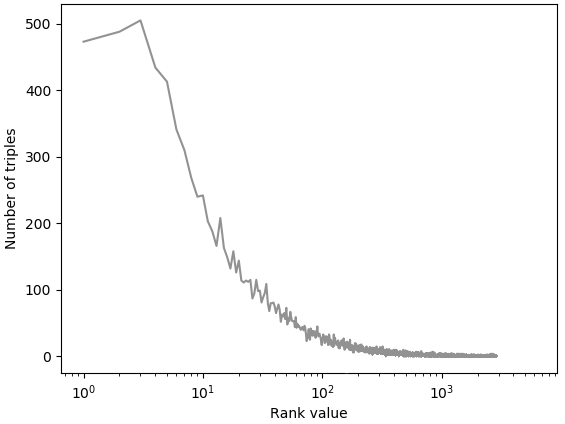
\includegraphics[scale=0.8]{img/num_triples_per_rank.png}
    \caption{
        Number of triples for each ranking position obtained by
        evaluating the best model found over the test set. The ranking
        positions range from 1 to 47,995.
    }
    \label{fig:num-triples-per-rank}
\end{figure}

The Figure \ref{fig:num-triples-per-rank} shows how the testing triples are
distributed over the possible ranking values.
As can be saw, the model is able to correctly assign an high rank to the
majority of the true facts.
\newpage

% evaluating different TMF topics
When looking at the statistics of the Polito Knowledge Graph, it is possible to
see how a large part of the entities are related
to the research topics, represented by the \emph{TMFResource} instances,
and connected to the publications by means of the \emph{dc:subject} relation.
In particular, as shown in Table \ref{tab:pkgsize}, almost a third of the
PKG edges link a publication to a subject extracted by TellMeFirst.

We wanted to evaluate how having a different number of \emph{TMFResource}
entities in the knowledge graph could have an impact on the trained model.
To do so, we built three new RDF graphs with a different numbers of topics
extracted by TellMeFrist for each publication.
In particular, we extracted three, seven and fourteen topics from each abstract.
Then, we trained the corresponding models by giving as input the datasets
created starting from such new graphs.
We used for the learning rate and the regularization hyperparameters the best
values found during the previous evaluation.


% table: Polito Knowledge Graph characteristics
\begin{table}[h]
    \footnotesize
    \centering
    \setlength\extrarowheight{5pt}
    \caption{
        Impact of the number of topics present in the RDF graph on the
        accuracy of the trained model.
    }
    \label{tab:tmfeval}

    \begin{tabularx}{1.0\textwidth}{ X | i  i  i }
            \toprule

            Number of topics extracted per-abstract & \textbf{3} & \textbf{7} & \textbf{14} \\
            Number of \emph{TMFResource} entities in the graph & 9.591 & 16.988 & 26.541 \\
            Number of \emph{dc:subject} edges & 45.423 & 107.093 & 212.226 \\
            MRR over test data & 0.103 & 0.0852 & 0.0671 \\
            HITS@15 & 31.5\% & 26.7\% & 20.3\% \\

            \bottomrule
    \end{tabularx}
\end{table}

% comment about table above
As can be seen from the results shown in Table \ref{tab:tmfeval}, the
different number of topics present in the three graphs greatly impact in the
accuracy of the resulting link prediction models.

% 3 topics
When we lowered the number of topics extracted to just three for each
publication, we saw an improvement in the evaluation metrics, however, this
did not lead to a better link prediction model.
In fact, the better ranking is a consequence of the less complex graph
structure: being the graph composed of almost half of the topic entities, is
more simple for the model to rank in a higher position the evaluated triples.
Moreover, there are more publications that shares the same topics, thus leading
to a model that is very capable of predicting the triples corresponding to
such topics as true facts during the evaluation over the test set.

% 14 topics
Instead, increasing the number of topics inside the graph led to a degradation
of the evaluation metrics. This can be easily be interpreted as a consequence
of the more complex graph structure obtained.
Moreover, the increase in the number of \emph{dc:subject} edges may have led
to a predominance of the topics when encoding the neighborhood representations
through the R-GCN, thus bringing a bias in the nodes embeddings obtained.
This could then impact on the results of the decoder, thus bringing to
more inaccurate predictions.
\newline

% empirical evaluation of the predicted triples
% esempi:
% 1) http://geranium-project.org/publications/11583/2584393

As we saw in the previous Chapter, the predicted triples are saved in the
form of a JSON file that is then used to load the new facts in the knowledge
base.
The predicted triples are the ones that received the highest score by the
DistMult decoder, thus being recognized as facts that, with an high likelihood,
should belong to the knowledge base.

Looking at the predictions obtained, we saw how the model was able to
truly characterize the graph entities, thus predicting meaningful
triples.
For example, the model predicted for a publication regarding
real-time tools for emergency management a new \emph{dc:subject} edge that
links such publication to a DBpedia resource\footnote{Entity URI: \url{http://dbpedia.org/resource/List_of_software_reliability_models}}
which collects the list of
software reliability models, which looks like an appropriate suggestion.
The model also predicted a new edge that connects the above publication to a
researcher whose main field of research is in integrated circuits for aircraft
applications, which is again a good prediction being the two topics fairly
related.
The above examples are just two among all the new, meaningful facts that
the model has been able to predict.
However, it is also true that there are predictions which are not correct, in
particular the ones regarding researchers who have a very low amount of
publications, for example students in their first years of PhD, or the ones
of publications that have a very misunderstandable abstracts, thus leading to
an incorrect topic extraction by TMF.
Some possible solutions to such issues are proposed in the next Chapter, where
are presented the possible future developments in this regard.



%%%%%%%%%%%%%%%%%%%%%%%%%%%%%%%%%%%%%%%%%%%%%%%%%%%%%%%%%%%%%%%%%%%%%%%%%%%%%%%%
% --------------------------- Conclusions and future work -------------------- %
%%%%%%%%%%%%%%%%%%%%%%%%%%%%%%%%%%%%%%%%%%%%%%%%%%%%%%%%%%%%%%%%%%%%%%%%%%%%%%%%
\chapter{Conclusions and Future Work}

%summary
In this work we presented an Academic Knowledge Graph built on top of the
metadata of the Politecnico di Torino publications.
Such knowledge graph links together researchers, publications, research
topics and scientific journals through the use of semantic relations.

We detailed the software architecture developed for the creation, enhancement
and visualization of such graph, particurlarly focusing our attention on the
enhancing phase.
In this regard, we used an approach based on Graph Convolutional
Networks to obtain an encoder model capable of embedding the nodes
characteristics into vector representations.
Such representations allowed us to predict new facts, so to complete the
information available in the knowledge base.
We used such predicted facts to empower a recommendation system whose
suggestions can be used by the researchers to explore new fields of
study, to discover other researchers who share the same research interests or
for retrieving other useful insights about their scientific community.

The scholarly data of any other academic institution could be used to
build a similar graph.
Moreover, metadata coming from different universities can be grouped
together to obtain a bigger and more complete knowledge graph,
representative of an even broader academic community. With this regard, we
look forward to obtain the metadata of other universities who
employ IRIS as their publications repository.
\newline

% future works
Regarding the technological aspects, we would like in future releases to
implement new factorization methods, testing wether or not the use of
different scoring functions can lead to even more accurate link prediction
models.
Moreover, one of the main limitations of the current implementation of the Enhancer
Module is that it is not able to predict new facts regarding entities that the
model has never seen during training. We would like to investigate in this
regard for new solutions based on the extension of the current encoder
architecture.
We would also like to test the use of input features generated using a
bag-of-words approach instead of the simple one-hot encoded vectors used for
the current model.

Another aspect that could be improved is the structure of the graph itself.
In the current implementation there are no dependencies or relations between
the research topics entities, however, in future releases we would like to add
a new layer of completeness by linking together the topics based on how they are
related to each other.
For example, \emph{Deep Learning} is a sub topic of \emph{Machine Learning},
which in turn is a sub topic of \emph{Artificial Intelligence}, but at the time
of writing this kind of information is not present in the Polito Knowledge Graph.
Such improvement could be achieved by leveraging the structured information
made available by the DBpedia project.
Moreover, the Dataset Builder could leverage such new information, keeping only
the specialized topics and discarding the most general ones. This could help to
obtain more characterized embeddings, as we already discussed in the previous
chapter.

Moreover, we would also like to collect some feedbacks from researchers,
who are the main users for whom our tool has been designed.
We could use such feedbacks to introduce a bias during the training phase, so
to penalize possible incorrect facts that have been wrongly predicted by the
Link Evaluator.

% conclusion
Our work has shown how is it possible to build new tools for the
sharing and dissemination of the knowledge produced by an academic institution
leveraging technologies of the Semantic Web and state-of-the-art machine
learning algorithms.
The recommendation system is a first step in the direction of
offering new tools to the researchers for exploring both new research fields
and the scientific community that study such fields.
Hopefully, this could lead to the contamination between researchers belonging
to different research areas but that are interested in the same research
topics, thus increasing the multidisciplinarity within the Politecnico di
Torino academic community.
Moreover, the Polito Knowledge Graph in its enhanced version is used to empower
as an expertise search engine made available to both the administration offices
of the Polito di Torino and to external parties, such as private organizations
or government agencies, who may be interested in finding expert profiles in a
given research area.


%%%%%%%%%%%%%%%%%%%%%%%%%%%%%%%%%%%%%%%%%%%%%%%%%%%%%%%%%%%%%%%%%%%%%%%%%%%%%%%%
% ------------------------------- Bigliography ------------------------------- %
%%%%%%%%%%%%%%%%%%%%%%%%%%%%%%%%%%%%%%%%%%%%%%%%%%%%%%%%%%%%%%%%%%%%%%%%%%%%%%%%
\bibliographystyle{IEEEtran}
\bibliography{references}

\end{document}
